\documentclass[a4paper,12pt]{article}

\usepackage{fancyhdr}
\usepackage{lastpage}
\usepackage{amsmath,amssymb,amsfonts,amsthm}
\usepackage{geometry}
\geometry{margin=2.5cm}
\usepackage{bm}
\usepackage{wrapfig}
\usepackage{braket}
\usepackage{mathtools}
\usepackage[noend, linesnumbered]{algorithm2e}
\SetKwComment{Comment}{$\triangleright$\ }{}
\RestyleAlgo{ruled}
\usepackage[skip=2pt]{parskip}  
\usepackage{tikz}
\usetikzlibrary{arrows.meta, positioning}
\usepackage{enumitem}
\usepackage{algorithm2e}
\usepackage{tcolorbox}
\usepackage[edges]{forest} % Para a árvore de busca


% ---- PREENCHA ----
\newcommand{\Lista}{2}
\newcommand{\Nome}{Isis Ardisson Logullo}
\newcommand{\NUSP}{7577410}
% -----------------------------

\newcommand{\N}{\mathbb{N}}
\newcommand{\bigO}[1]{\ensuremath{\mathcal{O}(#1)}}

\pagestyle{fancy}
\fancyhf{}
\fancyhead[L]{\Nome}
\fancyhead[R]{NUSP \NUSP}
\fancyfoot[L]{Lista \Lista}
\fancyfoot[C]{MAC0425}
\fancyfoot[R]{Página \thepage\ de \pageref{LastPage}}

\begin{document}

\section*{Exercício 1}

Dê as definições formais dos seguintes modelos de planejamento probabilístico:

\begin{enumerate}[label=\alph*)]
	\item MDP de horizonte finito
	\item MDP de horizonte infinito e descontado
	\item SSP
\end{enumerate}

\subsection*{Resposta:}

\bigskip

\textbf{a)} 

No modelo de horizonte finito, a tomada de decisão do agente é delimitada por um número fixo e conhecido de passos de tempo $N$ (também chamado de horizonte $H$).\\

Um MDP de Horizonte Finito é definido formalmente pela tupla:

$$\mathcal{M} = \langle S, A, P, R, N \rangle$$

onde:

$N \in \mathbb{N}$ é o horizonte temporal máximo do processo.\\

O objetivo é encontrar uma política que maximize o valor esperado da soma total de recompensas acumuladas ao longo dos $N$ passos:

$$U([s_0, s_1, \dots, s_N]) = \mathbb{E} \left[ \sum_{t=0}^{N-1} R(s_t, a_t, s_{t+1}) \right]$$

Propriedades Notáveis:
\begin{itemize}
	\item Não Estacionariedade da Política Ótima: A ação ótima a ser tomada depende explicitamente do tempo restante $t$. Por exemplo, a melhor escolha no passo $t=1$ (com $N-1$ passos restantes) pode ser diferente da melhor escolha no passo $t=N-1$ (com apenas 1 passo restante). Portanto, a política ótima é dependente do tempo: $\pi_t^*(s)$.
\end{itemize}

\bigskip

\textbf{b)}

No modelo de horizonte infinito, o processo continua indefinidamente ($N \to \infty$). Para evitar somas infinitas que não convergem e para modelar a preferência por recompensas imediatas em vez de futuras, introduz-se um fator de desconto.

Um MDP de Horizonte Infinito e Descontado é definido pela tupla:

$$\mathcal{M} = \langle S, A, P, R, \gamma \rangle$$

onde:

$\gamma \in [0, 1)$ é o fator de desconto.\\

O objetivo do agente é maximizar o valor esperado da soma de recompensas futuras descontadas:

$$U([s_0, s_1, s_2, \dots]) = \mathbb{E} \left[ \sum_{t=0}^{\infty} \gamma^t R(s_t, a_t, s_{t+1}) \right]$$

Propriedades Notáveis:
\begin{itemize}
	\item Convergência Matemáticas: Como $R$ é limitado e $\gamma < 1$, a série geométrica garante que a utilidade permaneça finita: $\sum_{t=0}^{\infty} \gamma^t R_{max} = \frac{R_{max}}{1 - \gamma}$.
	\item Estacionariedade da Política Ótima: O futuro restante a partir de qualquer estado $s$ é sempre infinito. Portanto, o tempo absoluto não altera a escolha ótima. A política ótima $\pi^*(s)$ é estacionária (mapeia o estado $s$ diretamente para a ação $a$, independentemente do instante $t$).
\end{itemize}

\bigskip

\textbf{c)}

O modelo de Caminho Estocástico mais Curtos (SSP) generaliza a busca do caminho mais curto para ambientes probabilísticos. O horizonte não é fixado a priori (como no caso finito) nem infinito, mas indefinido: o processo termina no momento em que o agente atinge um estado objetivo.

Um SSP é tipicamente formalizado pela tupla:

$$\mathcal{M} = \langle S, A, P, C, s_0, G \rangle$$

onde:

$G \subset S$ é um conjunto não vazio de estados objetivos (goal states), que são absorventes e possuem custo de saída zero: $P(g \mid g, a) = 1$ e $C(g, a) = 0$ para todo $g \in G$ e $a \in A$.\\

$C(s, a) > 0$ é a função de custo para a execução de uma ação $a$ em um estado $s \notin G$ (costuma-se usar custos estritamente positivos em vez de recompensas para penalizar passos adicionais).\\

$s_0 \in S$ é o estado inicial.

O objetivo é encontrar uma política que minimize o custo esperado acumulado até alcançar um estado de objetivo $g \in G$:

$$J^{\pi}(s) = \mathbb{E} \left[ \sum_{t=0}^{T-1} C(s_t, a_t) \,\,\Big\vert{}\,\, s_0 = s \right]$$

onde $T$ é uma variável aleatória que representa o instante de parada (primeira vez que $s_T \in G$).\\

Para garantir a existência de uma solução bem-definida e finita no SSP, a teoria exige duas premissas essenciais:

\begin{itemize}
	\item Existência de Política Própria (Proper Policy): Existe pelo menos uma política que alcança o objetivo $G$ a partir de qualquer estado inicial com probabilidade 1.
	\item Penalização de Políticas Impróprias: Toda política imprópria (uma política que corre o risco de nunca atingir $G$) incorre em um custo esperado infinito para os estados a partir dos quais não garante a chegada ao objetivo.
\end{itemize}


\section*{Exercício 2}

Dado um MDP de horizonte infinito e descontado, dê as definições para as
seguintes funções utilidade:

\begin{enumerate}[label=\alph*)]
	\item função valor de estado ( V(s) ).
	\item função valor de estado e ação ( Q(s,a) ).
\end{enumerate}


\subsection*{Resposta:}

\bigskip

Um Processo de Decisão de Markov (MDP) com horizonte infinito e fator de desconto trata da tomada de decisão em ambientes estocásticos onde a sequência de ações não possui um término fixo e as recompensas futuras têm menos peso do que as imediatas.\\

O Fator de Desconto ($\gamma$):

Antes de definir as funções de valor, vale destacar a utilidade aditiva descontada. Se o agente recebe uma sequência de recompensas $R_t, R_{t+1}, R_{t+2}, \dots$, o retorno total acumulado a partir do tempo $t$ é:

$$U([R_t, R_{t+1}, R_{t+2}, \dots]) = \sum_{k=0}^{\infty} \gamma^k R_{t+k}$$

Onde $\gamma \in [0, 1)$ é o fator de desconto. \\

Ele garante que a soma infinita convirja para um valor finito e reflete a preferência por recompensas mais imediatas.\\

\textbf{a)}

A função valor de estado $V^\pi(s)$ mede o retorno esperado descontado que o agente obterá ao começar no estado $s$ e, a partir dele, seguir a política $\pi$.

Matematicamente, é expressa como o valor esperado do retorno acumulado:

$$V^\pi(s) = \mathbb{E}_\pi \left[ \sum_{k=0}^{\infty} \gamma^k R_{t+k} \;\middle\vert{}\; S_t = s \right]$$


A utilidade de um estado $s$ sob uma política $\pi$ pode ser decomposta recursivamente usando a Equação de Bellman:

$$V^\pi(s) = R(s, \pi(s)) + \gamma \sum_{s'} P(s' \mid s, \pi(s)) \, V^\pi(s')$$

$R(s, a)$: É a recompensa imediata obtida ao executar a ação $a$ no estado $s$.\\

$P(s' \mid s, a)$: É a probabilidade de transição para o estado $s'$, dado que a ação $a$ foi tomada em $s$.\\

$\gamma \sum_{s'} P(s' \mid s, \pi(s)) V^\pi(s')$: É a soma ponderada das utilidades esperadas de todos os possíveis próximos estados $s'$, descontadas por $\gamma$.\\


A função valor ótima $V^*(s)$ representa o maior retorno esperado que se pode obter a partir do estado $s$, escolhendo a melhor ação possível:

$$V^*(s) = \max_{a \in A} \left[ R(s, a) + \gamma \sum_{s'} P(s' \mid s, a) \, V^*(s') \right]$$\\

\textbf{b)}

A função valor de estado-ação $Q^\pi(s, a)$ mede o retorno esperado descontado que o agente obterá ao começar no estado $s$, executar a ação $a$ no primeiro passo e, a partir de então, seguir a política $\pi$.

Matematicamente:

$$Q^\pi(s, a) = \mathbb{E}_\pi \left[ \sum_{k=0}^{\infty} \gamma^k R_{t+k} \;\middle\vert{}\; S_t = s, A_t = a \right]$$

A diferença fundamental em relação a $V(s)$ é que $Q(s,a)$ fixa a primeira ação como $a$, sem impor que $a$ venha da política $\pi(s)$.

A decomposição recursiva de Bellman para a função $Q$ é expressa por:

$$Q^\pi(s, a) = R(s, a) + \gamma \sum_{s'} P(s' \mid s, a) \, Q^\pi(s', \pi(s'))$$

No caso da política ótima $\pi^*$, a função $Q^*(s, a)$ representa o retorno máximo ao escolher $a$ em $s$ e agir otimamente a partir do próximo estado:

$$Q^*(s, a) = R(s, a) + \gamma \sum_{s'} P(s' \mid s, a) \max_{a'} Q^*(s', a')$$\\

\textbf{extra}

Relação entre $V(s)$ e $Q(s,a)$

As duas funções estão intimamente ligadas:
\begin{itemize}
	\item Obter $V(s)$ a partir de $Q(s,a)$ sob a política ótima:$$V^*(s) = \max_{a} Q^*(s, a)$$(O valor do estado é simplesmente o valor $Q$ da melhor ação disponível nele).
	\item Obter $Q(s,a)$ a partir de $V(s)$:$$Q^*(s, a) = R(s, a) + \gamma \sum_{s'} P(s' \mid s, a) \, V^*(s')$$
	\item Política Ótima $\pi^*(s)$:A política ótima pode ser extraída diretamente de $Q^*(s,a)$ sem a necessidade de conhecer o modelo de transição $P(s' \mid s, a)$:$$\pi^*(s) = \arg\max_{a} Q^*(s, a)$$
\end{itemize}


\section*{Exercício 3}

Dada uma política $p$ para um MDP de horizonte infinito descontado, qual é a equação que define a avaliação da política $p$ ?

\subsection*{Resposta:}

\bigskip

O processo de determinar a função valor $V^\pi(s)$ para uma política fixa $\pi$ é chamado de avaliação de política.

Para um MDP de horizonte infinito com fator de desconto $\gamma \in [0, 1)$, a equação que define a avaliação de uma política $\pi$ é a Equação de Expectativa de Bellman:

$$V^\pi(s) = R(s, \pi(s)) + \gamma \sum_{s'} P(s' \mid s, \pi(s)) \, V^\pi(s') \quad \forall s \in S$$

Onde:
\begin{itemize}
	\item $V^\pi(s)$: O valor (utilidade esperada descontada) de estar no estado $s$ e seguir a política $\pi$.
	\item $R(s, \pi(s))$: A recompensa imediata recebida por executar a ação prescrita pela política $\pi(s)$ no estado $s$.
	\item $\gamma$: O fator de desconto ($0 \le \gamma < 1$), que garante a convergência no horizonte infinito.
	\item $P(s' \mid s, \pi(s))$: A probabilidade de transição do estado $s$ para o estado $s'$ ao executar a ação $\pi(s)$.
	\item $\sum_{s'} P(s' \mid s, \pi(s)) \, V^\pi(s')$: O valor esperado do próximo estado $s'$.\\
\end{itemize}


Como a política $\pi$ é fixa, não há o operador de maximização ($\max_a$) na equação. Isso significa que, se houver $N$ estados no espaço de estados $S$:

\begin{itemize}
	\item A equação acima gera um sistema linear de $N$ equações a $N$ incógnitas (uma incógnita $V^\pi(s)$ para cada estado $s$).
	\item Esse sistema pode ser resolvido exatamente usando álgebra linear com complexidade de tempo $O(N^3)$, na forma matricial:
	$$\mathbf{V}^\pi = \mathbf{R}^\pi + \gamma \mathbf{P}^\pi \mathbf{V}^\pi \implies \mathbf{V}^\pi = (\mathbf{I} - \gamma \mathbf{P}^\pi)^{-1} \mathbf{R}^\pi$$
	\item Para ambientes com muitos estados (onde inverter a matriz é muito custoso), usa-se a resolução iterativa usando a avaliação iterativa de política, onde os valores são atualizados sucessivamente até a convergência:
	$$V_{k+1}(s) \leftarrow R(s, \pi(s)) + \gamma \sum_{s'} P(s' \mid s, \pi(s)) \, V_k(s')$$
\end{itemize}


\section*{Exercício 4}

Descreva a Equação de Otimalidade da Bellman para MDPs de horizonte infinito descontado.


\subsection*{Resposta:}

\bigskip

A Equação de Otimalidade de Bellman é o pilar fundamental para caracterizar o comportamento de um agente racional em um Processo de Decisão de Markov (MDP) de horizonte infinito descontado.\\

Ela estabelece a relação de consistência que a função valor ótima $V^*(s)$ — ou a função $Q$ ótima $Q^*(s,a)$ — deve satisfazer quando o agente escolhe a melhor ação possível em todos os passos.\\

A função valor ótima $V^*(s)$ representa o retorno total descontado esperado ao começar no estado $s$ e agir otimamente a partir de então.\\

$$V^*(s) = \max_{a \in A(s)} \left[ R(s, a) + \gamma \sum_{s'} P(s' \mid s, a) \, V^*(s') \right] \quad \forall s \in S$$

Onde:
\begin{itemize}
	\item $V^*(s)$: A utilidade máxima esperada de estar no estado $s$.
	\item $\max_{a \in A(s)}$: O operador de seleção que busca a ação $a$ disponível no estado $s$ que maximiza o retorno total esperado.
	\item $R(s, a)$: A recompensa imediata obtida ao tomar a ação $a$ no estado $s$.
	\item $\gamma$: O fator de desconto ($0 \le \gamma < 1$), que assegura que a soma infinita convirja para um valor finito e prioriza recompensas mais próximas.
	\item $P(s' \mid s, a)$: A probabilidade de transitar para o estado $s'$ após executar a ação $a$ no estado $s$.
	\item $\sum_{s'} P(s' \mid s, a) \, V^*(s')$: A utilidade média esperada do próximo estado $s'$, ponderada pelas probabilidades do ambiente.
\end{itemize}

A essência da equação é o Princípio da Otimalidade de Bellman:

A utilidade ótima de um estado $s$ é igual à recompensa imediata máxima recebida pela melhor ação $a$, somada ao valor ótimo descontado dos estados subsequentes $s'$ resultantes dessa ação.\\

Se expressarmos a otimalidade em termos do valor da dupla estado-ação ($Q^*$), a equação toma a seguinte forma:

$$Q^*(s, a) = R(s, a) + \gamma \sum_{s'} P(s' \mid s, a) \max_{a'} Q^*(s', a')$$

Neste caso, a otimalidade no próximo estado $s'$ é garantida pela escolha do maior valor entre todas as ações $a'$ disponíveis em $s'$ ($\max_{a'} Q^*(s', a')$).\\

I. Não Linearidade\\

Ao contrário da equação de avaliação de política (que é um sistema de equações lineares), a equação de otimalidade contém o operador $\max$, o que a torna não linear. Por esse motivo, não é possível resolvê-la diretamente com métodos de álgebra linear tradicional (como a inversão de matrizes).\\

II. Existência e Unicidade da Solução\\

Para qualquer MDP descontado de horizonte infinito com $0 \le \gamma < 1$, existe uma única solução $V^*$ para o sistema de equações de Bellman. A aplicação iterativa do operador de otimalidade forma uma contração (Contraction Mapping), garantindo que os métodos convergiram para o mesmo valor fixo.\\

III. Extração da Política Ótima ($\pi^*$)\\

Uma vez calculados os valores de $V^*(s)$ para todos os estados, a política ótima $\pi^*$ é obtida escolhendo, em cada estado $s$, a ação que atinge o máximo na equação:

$$\pi^*(s) = \arg\max_{a \in A(s)} \left[ R(s, a) + \gamma \sum_{s'} P(s' \mid s, a) \, V^*(s') \right]$$

Se a função $Q^*(s,a)$ for conhecida, a escolha simplifica-se para:

$$\pi^*(s) = \arg\max_{a \in A(s)} Q^*(s, a)$$

Dois algoritmos clássicos são apresentados para resolver a Equação de Otimalidade de Bellman:\\

1) Iteração de Valor: \\

Aplica a equação de otimalidade como uma regra de atualização iterativa até que os valores de $V(s)$ convirjam:

$$V_{k+1}(s) \leftarrow \max_{a} \left[ R(s, a) + \gamma \sum_{s'} P(s' \mid s, a) \, V_k(s') \right]$$

2) Iteração de Política:\\

Alterna entre avaliar uma política fixa (sistema linear) e melhorá-la de forma gulosa com base nos valores calculados.



\section*{Exercício 5}

Dê as definições para os seguintes tipos de política:

\begin{enumerate}[label=\alph*)]
	\item política parcial
	\item política própria
	\item política gulosa
	\item política ótima
\end{enumerate}	

\subsection*{Resposta:}

\bigskip

Uma política $\pi$ é uma regra de decisão que especifica qual ação o agente deve tomar em cada estado do ambiente. Formamente, é uma função ou mapeamento $\pi: S \to A$.\\

\textbf{a)}

Uma política parcial é uma função que não define ações para todos os estados possíveis do MDP, estando especificada apenas para um subconjunto do espaço de estados $S_{definido} \subset S$.\\

Em ambientes muito grandes, na busca em árvore online ou no uso de algoritmos de planejamento parcial (como em Real-Time Dynamic Programming - RTDP), calcula-se a tomada de decisão apenas para os estados que o agente é capaz de alcançar a partir do seu estado atual dentro de certo horizonte, deixando os estados irrelevantes ou inacessíveis sem uma ação mapeada.\\


Em contraste, uma política completa especifica uma ação válida $\pi(s)$ para todos os estados $s \in S$ que o agente possa eventualmente visitar.  \\

\textbf{b)}

Uma política própria é uma política que garante atingir um estado terminal (ou estado meta) com probabilidade 1, independentemente de qual seja o estado inicial do agente.  \\

Essa definição aplica-se especificamente a MDPs que contêm estados de término/meta — um modelo frequentemente tratado como o problema do Caminho Mínimo Estocástico (SSP). \\

Uma política $\pi$ é dita própria se, a partir de qualquer estado $s \in S$, o limite da probabilidade de o agente alcançar o estado meta $s_g \in G$ à medida que o tempo $t \to \infty$ é igual a 1:  

$$\lim_{t \to \infty} P(S_t \in G \mid S_0 = s, \pi) = 1$$

Política Imprópria: Se existir ao menos um estado inicial a partir do qual a política corra o risco de prender o agente em um loop infinito sem nunca alcançar o estado terminal, essa política é classificada como imprópria. \\

\textbf{c)}

Uma política gulosa é aquela que seleciona, em cada estado $s$, a ação que maximiza a utilidade esperada de curto prazo em relação a uma função valor atual/arbitrária $V(s)$ ou $Q(s,a)$.\\

Formulação com Função Valor de Estado $V(s)$:

$$\pi_{gulosa}(s) = \arg\max_{a \in A(s)} \left[ R(s, a) + \gamma \sum_{s'} P(s' \mid s, a) \, V(s') \right]$$

Formulação com Função Valor de Estado-Ação $Q(s,a)$:

$$\pi_{gulosa}(s) = \arg\max_{a \in A(s)} Q(s, a)$$

O conceito de política gulosa é central no algoritmo de Iteração de Política. A cada passo de melhoria da política, o agente deriva uma nova política gulosa a partir da função valor calculada na etapa de avaliação da política anterior.\\

\textbf{d)}

A política ótima, denotada por $\pi^*$, é a política que maximiza o retorno total descontado esperado a partir de qualquer estado inicial $s \in S$.  \\

Uma política $\pi^*$ é ótima se a sua função valor $V^{\pi^*}(s)$ for estritamente superior ou igual à função valor $V^\pi(s)$ de qualquer outra política $\pi$, para todos os estados $s \in S$:

$$V^{\pi^*}(s) \ge V^\pi(s) \quad \forall \pi, \; \forall s \in S$$

Uma política ótima é obtida agindo de forma gulosa em relação à função valor ótima $V^*(s)$:

$$\pi^*(s) = \arg\max_{a \in A(s)} \left[ R(s, a) + \gamma \sum_{s'} P(s' \mid s, a) \, V^*(s') \right]$$

Unicidade e Estacionariedade no Horizonte Infinito:\\

Demonstra-se que, para MDPs descontados de horizonte infinito, sempre existe pelo menos uma política ótima que é estática/estacionária e determinística — ou seja, a ação ideal depende apenas do estado atual $s$, e não do tempo decorrido ou do histórico do agente. 



\section*{Exercício 6}

Considere o MDP ilustrado da figura abaixo.

\begin{figure}[ht]
	\centering
	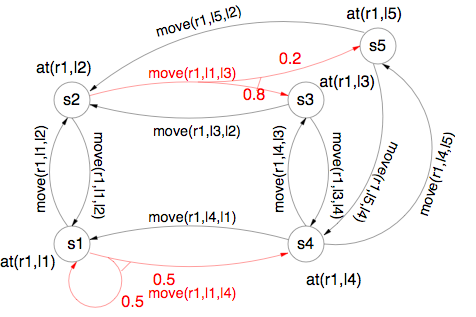
\includegraphics[width=1\textwidth]{imagem6.png}
\end{figure}

\newpage

Considere a função utilidade local como R(s) – C(s,a) (isto é, recompensa menos o custo); sendo
que definimos a função custo para os pares estado/ação, insto é C(s,a), como:
\begin{itemize}
	\item C(s,wait) = 0 para todo estado s ,
	\item C(s,a) = 1 para toda ação “horizontal” ,
	\item C(s,a) = 100 para toda ação “vertical” ,
\end{itemize}

e a função recompensa para o estado, sendo R(s) = 0 para todo estado s, exceto para os estados
s4 e s5 que são definidas por:
\begin{itemize}
	\item R(s4) = 100
	\item R(s5) = -100
\end{itemize}

Considere também que é dada a política p especificada conforme a tabela abaixo.

\begin{table}[h!]
	\centering
	\begin{tabular}{|c|c|}
		\hline
		\textbf{Estado $s$} & \textbf{Ação $\pi(s)$} \\ \hline
		$s_1$ & $\text{move}(r1, l1, l2)$ \\ \hline
		$s_2$ & $\text{move}(r1, l2, l3)$ \\ \hline
		$s_3$ & $\text{move}(r1, l3, l4)$ \\ \hline
		$s_4$ & $\text{wait}$ \\ \hline
		$s_5$ & $\text{move}(r1, l5, l4)$ \\ \hline
	\end{tabular}
\end{table}

\subsection*{Resposta:}

\bigskip

Horizonte e Desconto: 

Assumimos $\gamma = 1$ (ou sem desconto explícito indicado para as iterações).  \\

Recompensas e Custos: 
\begin{itemize}
	\item $R(s) - C(s,a)$:  $R(s_4) = 100$, $R(s_5) = -100$, e $R(s_1) = R(s_2) = R(s_3) = 0$.
	\item Custo de ações: $C(wait) = 0$, $C(\text{horizontal}) = 1$, $C(\text{vertical}) = 100$.
	\item Recompensa Líquida $R'(s,a) = R(s) - C(s,a)$:
	\begin{itemize}
		\item $R'(s_1, move(r1, l1, l2)) = 0 - 1 = -1$
		\item $R'(s_2, move(r1, l2, l3)) = 0 - 1 = -1$
		\item $R'(s_3, move(r1, l3, l4)) = 0 - 1 = -1$
		\item $R'(s_4, wait) = 100 - 0 = 100$
		\item $R'(s_5, move(r1, l5, l4)) = -100 - 1 = -101$ \\
	\end{itemize}
\end{itemize}

Probabilidades de Transição dada a política $\pi$:
\begin{itemize}
	\item Em $s_1$: $\pi(s_1) = move(r1, l1, l2)$ leva a $s_2$ com $P=0.8$ e a $s_3$ com $P=0.2$.
	\item Em $s_2$: $\pi(s_2) = move(r1, l2, l3)$ leva a $s_3$ com $P=1.0$.
	\item Em $s_3$: $\pi(s_3) = move(r1, l3, l4)$ leva a $s_4$ com $P=0.5$ e $s_1$ com $P=0.5$.
	\item Em $s_4$: $\pi(s_4) = wait$ permanece em $s_4$ com $P=1.0$.
	\item Em $s_5$: $\pi(s_5) = move(r1, l5, l4)$ leva a $s_4$ com $P=1.0$.  \\
\end{itemize}


Iterações da Avaliação de Política ($V_0(s) = 0$ para todo $s$):
\begin{itemize}
	\item $1^{\text{a}}$ Iteração ($k=1$):
	\begin{itemize}
		\item $V^1(s_1) = -1 + [0.8(0) + 0.2(0)] = -1$
		\item $V^1(s_2) = -1 + 1.0(0) = -1$
		\item $V^1(s_3) = -1 + [0.5(0) + 0.5(0)] = -1$ 
		\item $V^1(s_4) = 100 + 1.0(0) = 100$
		\item $V^1(s_5) = -101 + 1.0(0) = -101$
	\end{itemize}
	\item $2^{\text{a}}$ Iteração ($k=2$):
	\begin{itemize}
		\item $V^2(s_1) = -1 + [0.8(-1) + 0.2(-1)] = -1 - 1 = -2$
		\item $V^2(s_2) = -1 + 1.0(-1) = -2$ 
		\item $V^2(s_3) = -1 + [0.5(100) + 0.5(-1)] = -1 + 49.5 = 48.5$
		\item $V^2(s_4) = 100 + 1.0(100) = 200$
		\item $V^2(s_5) = -101 + 1.0(100) = -1$
	\end{itemize}
	\item $3^{\text{a}}$ Iteração ($k=3$):
	\begin{itemize}
		\item $V^3(s_1) = -1 + [0.8(-2) + 0.2(48.5)] = -1 + [-1.6 + 9.7] = 7.1$
		\item $V^3(s_2) = -1 + 1.0(48.5) = 47.5$
		\item $V^3(s_3) = -1 + [0.5(200) + 0.5(-2)] = -1 + [100 - 1] = 98$
		\item $V^3(s_4) = 100 + 1.0(200) = 300$
		\item $V^3(s_5) = -101 + 1.0(200) = 99$
	\end{itemize}
\end{itemize}
                          
\begin{table}[h!]
	\centering
	\begin{tabular}{|c|c|c|c|}
		\hline
		\textbf{Estado $s$} & \textbf{$V^\pi$ (1ª iteração)} & \textbf{$V^\pi$ (2ª iteração)} & \textbf{$V^\pi$ (3ª iteração)} \\ \hline
		$s_1$ & $-1$ & $-2$ & $7,1$ \\ \hline
		$s_2$ & $-1$ & $-2$ & $47,5$ \\ \hline
		$s_3$ & $-1$ & $48,5$ & $98$ \\ \hline
		$s_4$ & $100$ & $200$ & $300$ \\ \hline
		$s_5$ & $-101$ & $-1$ & $99$ \\ \hline
	\end{tabular}
\end{table}

\section*{Exercício 7}

Considere um cenário onde um robô vigilante deve permanecer num corredor de um prédio, sem
atrapalhar a passagem das pessoas. Uma vez que do lado esquerdo desse corredor existem
portas, o robô atrapalha menos quando permanece do lado direito. Além disso, quando o robô se
desloca, a posição desejada é alcançada com probabilidade 0.7 (e com probabilidade 0.3, ele
continua na mesma posição em que estava). Em cada instante, o robô deve decidir qual a melhor
ação: permanecer onde está ou se mover para direita ou esquerda. Este problema pode ser
modelado por um MDP $<$S,A,P,R,C$>$ cujo grafo de transição de estados é dado pela Figura 4. As
arestas são rotuladas pelas ações \textit{permanecer, paraesq e paradir}. E suas probabilidades de
transição. Ovais são rotuladas pelos estados e o valor de recompensa.

\begin{figure}[ht]
	\centering
	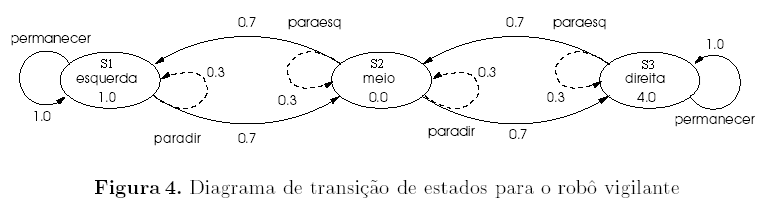
\includegraphics[width=1\textwidth]{imagem7.png}
\end{figure}

Notem que existem três possíveis estados no conjunto S:
\begin{itemize}
	\item s1: Loc = esquerda
	\item s2: Loc = meio
	\item s3: Loc = direita
\end{itemize}

O conjunto de ações A = \{\textit{permanecer, paraesq, paradir}\} especifica as possíveis ações do robô; P
é a função de transição de estados probabilística, dada por:
\begin{itemize}
	\item P(s1| \textit{permanecer}, s1) = 1.0
	\item P(s1| \textit{paradir}, s1) = 0.3
	\item P(s2| \textit{paradir}, s1) = 0.7
	\item P(s2| \textit{paradir}, s2) = 0.3
	\item P(s3| \textit{paradir}, s2) = 0.7
	\item P(s2| \textit{paraesq}, s2) = 0.3
	\item P(s1| \textit{paraesq}, s2) = 0.7
	\item P(s3| \textit{permanecer}, s3) = 1
	\item P(s3| \textit{paraesq}, s3) = 0.3
	\item P(s2| \textit{paraesq}, s3) = 0.7
\end{itemize}

R é a função que associa recompensas a estados (de modo que posições preferidas sejam
melhor recompensadas):

\begin{itemize}
	\item R(s1) = 1.0
	\item R(s2) = 0.0
	\item R(s3) = 4.0
\end{itemize}

e, finalmente, C é a função custo das ações do robô (de modo que ações preferidas tenham custo
menor):

\begin{itemize}
	\item C(permanecer)=0
	\item C(paraesq)=1
	\item C(paradir)=1
\end{itemize}

Considere a política inicial:

\begin{table}[h!]
	\centering
	\begin{tabular}{|c|c|}
		\hline
		\textbf{Estado} & \textbf{Ação} \\ \hline
		$s_1$ & $\textit{permanecer}$ \\ \hline
		$s_2$ & $\textit{paradir}$ \\ \hline
		$s_3$ & $\textit{permanecer}$ \\ \hline
	\end{tabular}
\end{table}

Sabendo que neste MDP queremos maximizar o valor esperado acumulado descontado de R-C,
calcule (manualmente) a política ótima estacionária, com $\gamma = 0.9$, usando o algoritmo de iteração
de política especificado a seguir. Note que o algoritmo usa a ideia mas simples de resolução de
sistema de equações lineares (Aula 17, slide 58).

\begin{algorithm}[H]
	\SetAlgoLined
	\caption{Iteração-de-Política($S, A, P, R, C, \gamma$)}
	
	$\pi \leftarrow \emptyset$ \;
	Selecione qualquer $\pi' \neq \emptyset$ \tcp*{Política inicial dada}
	
	\While{$\pi' \neq \pi$}{
		$\pi \leftarrow \pi'$ \;
		\ForEach{$s \in S$}{
			$E_{\pi}(s) \leftarrow$ solução do sistema de equações: \;
			$E_{\pi}(s) = R(s) - C(\pi(s)) + \gamma \sum_{s' \in S} P(s' \mid s, \pi(s)) E_{\pi}(s')$ \;
		}
		\ForEach{$s \in S$}{
			\eIf{$\exists a \in A \mid E_{\pi}(s) < R(s) - C(a) + \gamma \sum_{s' \in S} P(s' \mid s, a) E_{\pi}(s')$}{
				$\pi'(s) \leftarrow a$ \;
			}{
				$\pi'(s) \leftarrow \pi(s)$ \;
			}
		}
	}
	\Return $\pi$ \;
\end{algorithm}

\subsection*{Resposta:}

\bigskip


\begin{itemize}
	\item Conjunto de Estados: $S = \{s_1, s_2, s_3\}$
	\item Conjunto de Ações: $A = \{\textit{permanecer}, \textit{paraesq}, \textit{paradir}\}$
	\item Fator de Desconto: $\gamma = 0.9$
	\item Recompensas dos Estados $R(s)$:
	\[
	R(s_1) = 1.0, \quad R(s_2) = 0.0, \quad R(s_3) = 4.0
	\]
	\item Custos das Ações $C(a)$:
	\[
	C(\textit{permanecer}) = 0, \quad C(\textit{paraesq}) = 1, \quad C(\textit{paradir}) = 1
	\]
	\item Política Inicial ($\pi_0$):
	\[
	\pi_0(s_1) = \textit{permanecer}, \quad \pi_0(s_2) = \textit{paradir}, \quad \pi_0(s_3) = \textit{permanecer}
	\]
\end{itemize}


\subsubsection*{1ª Iteração: Avaliação da Política ($\pi_0$)}
A equação de avaliação de política é dada por:
\[
E_\pi(s) = R(s) - C(\pi(s)) + \gamma \sum_{s' \in S} P(s' \mid s, \pi(s)) E_\pi(s')
\]

\begin{enumerate}
	\item \textbf{Para $s_1$} com $\pi_0(s_1) = \textit{permanecer}$ ($C=0, P(s_1 \mid s_1) = 1.0$):
	\[
	E_\pi(s_1) = 1.0 - 0 + 0.9 (1.0 \cdot E_\pi(s_1)) \implies 0.1 E_\pi(s_1) = 1.0 \implies \mathbf{E_\pi(s_1) = 10}
	\]
	
	\item \textbf{Para $s_3$} com $\pi_0(s_3) = \textit{permanecer}$ ($C=0, P(s_3 \mid s_3) = 1.0$):
	\[
	E_\pi(s_3) = 4.0 - 0 + 0.9 (1.0 \cdot E_\pi(s_3)) \implies 0.1 E_\pi(s_3) = 4.0 \implies \mathbf{E_\pi(s_3) = 40}
	\]
	
	\item \textbf{Para $s_2$} com $\pi_0(s_2) = \textit{paradir}$ ($C=1, P(s_2 \mid s_2) = 0.3, P(s_3 \mid s_2) = 0.7$):
	\[
	E_\pi(s_2) = 0.0 - 1.0 + 0.9 [0.3 E_\pi(s_2) + 0.7 E_\pi(s_3)]
	\]
	Substituindo $E_\pi(s_3) = 40$:
	\[
	E_\pi(s_2) = -1.0 + 0.27 E_\pi(s_2) + 0.63(40) \implies 0.73 E_\pi(s_2) = 24.2 \implies \mathbf{E_\pi(s_2) \approx 33.15}
	\]
\end{enumerate}

\subsubsection*{1ª Iteração: Melhoria da Política}
Avaliamos a utilidade esperada $Q(s, a) = R(s) - C(a) + \gamma \sum_{s'} P(s' \mid s, a) E_\pi(s')$ para cada ação:

\begin{itemize}
	\item \textbf{No Estado $s_1$:}
	\begin{align*}
		Q(s_1, \textit{permanecer}) &= 1.0 - 0 + 0.9(1.0 \times 10) = \mathbf{10.0} \\
		Q(s_1, \textit{paradir}) &= 1.0 - 1 + 0.9[0.3(10) + 0.7(33.15)] = 0.9(26.205) = \mathbf{23.58}
	\end{align*}
	Como $23.58 > 10.0$, atualizamos $\pi_1(s_1) = \mathbf{\textit{paradir}}$.
	
	\item \textbf{No Estado $s_2$:}
	\begin{align*}
		Q(s_2, \textit{paradir}) &= 0.0 - 1 + 0.9[0.3(33.15) + 0.7(40)] = \mathbf{33.15} \\
		Q(s_2, \textit{paraesq}) &= 0.0 - 1 + 0.9[0.7(10) + 0.3(33.15)] = \mathbf{14.25}
	\end{align*}
	Mantemos $\pi_1(s_2) = \mathbf{\textit{paradir}}$.
	
	\item \textbf{No Estado $s_3$:}
	\begin{align*}
		Q(s_3, \textit{permanecer}) &= 4.0 - 0 + 0.9(1.0 \times 40) = \mathbf{40.0} \\
		Q(s_3, \textit{paraesq}) &= 4.0 - 1 + 0.9[0.7(33.15) + 0.3(40)] = \mathbf{34.68}
	\end{align*}
	Mantemos $\pi_1(s_3) = \mathbf{\textit{permanecer}}$.
\end{itemize}

A nova política obtida é $\pi_1 = \{\textit{paradir}, \textit{paradir}, \textit{permanecer}\}$. Como $\pi_1 \neq \pi_0$, seguimos para a segunda iteração.


\subsubsection*{2ª Iteração: Avaliação da Nova Política ($\pi_1$)}

\begin{enumerate}
	\item \textbf{Para $s_3$:} $\mathbf{E_\pi(s_3) = 40}$
	\item \textbf{Para $s_2$:} $\mathbf{E_\pi(s_2) \approx 33.15}$
	\item \textbf{Para $s_1$} com $\pi_1(s_1) = \textit{paradir}$ ($C=1, P(s_1 \mid s_1) = 0.3, P(s_2 \mid s_1) = 0.7$):
	\[
	E_\pi(s_1) = 1.0 - 1.0 + 0.9[0.3 E_\pi(s_1) + 0.7 E_\pi(s_2)]
	\]
	\[
	E_\pi(s_1) = 0.27 E_\pi(s_1) + 0.63(33.15) \implies 0.73 E_\pi(s_1) = 20.8845 \implies \mathbf{E_\pi(s_1) \approx 28.61}
	\]
\end{enumerate}

\subsubsection*{2ª Iteração: Melhoria da Política}
\begin{itemize}
	\item \textbf{No Estado $s_1$:}
	\begin{align*}
		Q(s_1, \textit{permanecer}) &= 1.0 - 0 + 0.9(1.0 \times 28.61) = \mathbf{26.75} \\
		Q(s_1, \textit{paradir}) &= 0.0 + 0.9[0.3(28.61) + 0.7(33.15)] = \mathbf{28.61}
	\end{align*}
	Ação $\textit{paradir}$ permanece como a melhor opção.
\end{itemize}

Como $\pi_2 = \pi_1$, o algoritmo convergiu.

\subsubsection*{3. Resultado Final}

A política ótima estacionária $\pi^*$ encontrada pelo algoritmo é:

\begin{table}[h!]
	\centering
	\begin{tabular}{|c|c|}
		\hline
		\textbf{Estado $s$} & \textbf{Ação Ótima $\pi^*(s)$} \\ \hline
		$s_1$ & $\textit{paradir}$ \\ \hline
		$s_2$ & $\textit{paradir}$ \\ \hline
		$s_3$ & $\textit{permanecer}$ \\ \hline
	\end{tabular}
\end{table}


\section*{Exercício 8}

Explique a diferença entre os algoritmos Iteração de Valor (IV), Iteração de Política (IP) e Real Time Dynamic Programming (RTDP)


\subsection*{Resposta:}

\bigskip


Os três algoritmos utilizam o princípio da Programação Dinâmica para resolver Processos de Decisão de Markov (MDPs), mas diferem na forma como atualizam as funções de valor e na maneira como exploram o espaço de estados:

Iteração de Valor:\\
\begin{itemize}
	\item Mecanismo: Atualiza diretamente a função valor dos estados $V(s)$ através da aplicação iterativa da Equação de Otimalidade de Bellman.
	\item Funcionamento: Em cada iteração, recalcula o valor $V(s)$ para todos os estados $s \in S$ aplicando o operador de maximização sobre todas as ações possíveis:
	\[
	V_{k+1}(s) \leftarrow \max_{a \in A} \left[ R(s,a) + \gamma \sum_{s'} P(s' \mid s, a) V_k(s') \right]
	\]
	\item Característica: Não mantém nem avalia uma política explícita durante as iterações. A política ótima só é extraída de forma gulosa ao final, quando $V(s)$ convergir.\\
\end{itemize}

Iteração de Política:\\
\begin{itemize}
	\item Mecanismo: Mantém uma política explícita $\pi$ e alterna entre duas etapas até a convergência:
	\begin{enumerate}
		\item Avaliação de Política: Calcula exatamente (ou aproxima) a função valor $V^\pi(s)$ para a política atual $\pi$, resolvendo um sistema de equações lineares:
		\[
		E_\pi(s) = R(s) - C(\pi(s)) + \gamma \sum_{s'} P(s' \mid s, \pi(s)) E_\pi(s')
		\]
		\item Melhoria de Política: Atualiza a política $\pi(s)$ de forma gulosa em relação aos valores $V^\pi(s)$ recém-calculados.
	\end{enumerate}
	\item Característica: Requer geralmente menos iterações que a Iteração de Valor para convergir, porém cada iteração é mais custosa computacionalmente devido à resolução do sistema de equações lineares.\\
\end{itemize}

Real-Time Dynamic Programming (RTDP):\\
\begin{itemize}
	\item Mecanismo: É uma variante assíncrona da Iteração de Valor focada no planejamento em tempo real durante a execução ou simulação de episódios.
	\item Funcionamento: Em vez de realizar uma varredura completa atualizando todos os estados do ambiente (o que é inviável para espaços de estados imensos), o RTDP realiza atualizações de Bellman apenas nos estados visitados ao longo de trajetórias simuladas a partir de um estado inicial até o estado meta.
	\item Característica: Concentra os recursos computacionais exclusivamente nos estados que são relevantes e alcançáveis sob a política atual, sem a necessidade de processar todo o espaço de estados $S$.
\end{itemize}



\begin{table}[h!]
	\centering
	\begin{tabular}{|l|p{4cm}|p{4.5cm}|}
		\hline
		\textbf{Algoritmo} & \textbf{O que é atualizado} & \textbf{Varredura do Espaço de Estados} \\ \hline
		\textbf{Iteração de Valor (IV)} & Função valor $V(s)$ & Varredura completa ($s \in S$) \\ \hline
		\textbf{Iteração de Política (IP)} & Política $\pi(s)$ e Valor $V^\pi(s)$ & Varredura completa ($s \in S$) \\ \hline
		\textbf{RTDP} & Função valor $V(s)$ & Amostrada/Focada em trajetórias relevantes \\ \hline
	\end{tabular}
\end{table}

\section*{Exercício 9}

Dê uma definição (informal) de Aprendizado por Reforço.


\subsection*{Resposta:}

\bigskip

O Aprendizado por Reforço é um paradigma de aprendizado de máquina no qual um agente aprende a tomar decisões em um ambiente dinâmico por meio de tentativa e erro. \\

Diferente do aprendizado supervisionado, o agente não recebe instruções explícitas sobre qual ação tomar em cada situação; em vez disso, ele executa ações no ambiente e recebe retornos numéricos chamados de recompensas (positivas) ou punições (negativas).\\

O objetivo principal do agente é aprender uma política de comportamento que maximize a quantidade total de recompensa acumulada ao longo do tempo.\\


Principais Características:\\

\begin{itemize}
	\item Aprendizado sem Supervisor: Não há um professor para rotular as ações corretas ou incorretas. O sinal de feedback indica apenas quão bom ou ruim foi o resultado de uma ação.
	\item Recompensa Atrasada: Uma ação tomada no presente pode afetar não apenas a recompensa imediata, mas também todas as recompensas futuras.
	\item Exploration vs. Exploitation: Para obter altas recompensas, o agente deve preferir ações que já testou no passado e se mostraram eficazes (\textit{explotação}). No entanto, para descobrir tais ações, ele precisa experimentar opções nunca antes testadas (\textit{exploração}).
\end{itemize}

\section*{Exercício 10}

Explique a diferença entre os seguintes conceitos de Aprendizado por Reforço (AR):

\begin{enumerate}[label=\alph*)]
	\item Predição Vs Controle
	\item \textit{Model-Based} Vs \textit{Model-Free}
	\item Aprendizado por Reforço \textit{on-policy} Vs \textit{off-policy}
\end{enumerate}


\subsection*{Resposta:}

\bigskip


\textbf{a)}


A distinção entre Predição e Controle aborda duas metas fundamentais no aprendizado por reforço:

\begin{itemize}
	\item Predição (Avaliação de Política):
	\begin{itemize}
		\item Determinar a função de valor $V^\pi(s)$ (ou $Q^\pi(s,a)$) para uma política $\pi$ fixa e dada.
		\item O problema responde à pergunta: "Quão boa é essa política específica?". O agente observa as transições e recompensas geradas ao seguir a política $\pi$ e estima o retorno esperado para cada estado $s$, sem tentar modificar a política durante o processo.
	\end{itemize}
	
	\item Controle (Otimização de Política):
	\begin{itemize}
		\item Encontrar a política ótima $\pi^*$ que maximiza o retorno acumulado esperado no ambiente.
		\item O problema responde à pergunta: "Qual é a melhor forma de agir?". Envolve combinar a avaliação de política com a melhoria contínua da política (como no paradigma de \textit{Generalized Policy Iteration}), buscando selecionar as ações que levam aos melhores resultados de longo prazo.\\
	\end{itemize}
\end{itemize}



\textbf{b)} 

Essa classificação diz respeito ao conhecimento ou aprendizado prévio do agente sobre as dinâmicas do ambiente:

\begin{itemize}
	\item Model-Based 
	\begin{itemize}
		\item O agente possui ou aprende um modelo explícito do ambiente. Esse modelo consiste no modelo de transição $P(s' \mid s, a)$ (a probabilidade de ir para o estado $s'$ ao tomar a ação $a$ no estado $s$) e na função de recompensa $R(s, a)$.
		\item Permite que o agente faça planejamento (como simular trajetórias hipotéticas antes de agir) e use técnicas de programação dinâmica. No entanto, aprender ou armazenar um modelo exato do ambiente pode ser extremamente custoso ou inviável em termos computacionais para espaços de estados grandes.
	\end{itemize}
	
	\item Model-Free
	\begin{itemize}
		\item O agente não possui e nem tenta aprender as probabilidades de transição $P(s' \mid s, a)$ ou o modelo $R(s,a)$.
		\item Em vez de planejar com base no ambiente, o agente aprende diretamente funções de valor (como $Q(s,a)$ no \textit{Q-Learning}) ou políticas ótimas a partir do feedback direto de suas interações reais (amostras). É ideal para ambientes complexos ou estocásticos onde modelar as regras exatas do mundo é inviável.\\
	\end{itemize}
\end{itemize}


\textbf{c)} 

Esta diferença refere-se ao relacionamento entre a política que o agente utiliza para gerar ações no ambiente e a política que ele está tentando avaliar ou otimizar:

\begin{itemize}
	\item On-Policy 
	\begin{itemize}
		\item O agente aprende o valor da política que ele está de fato executando para explorar o ambiente.
		\item A política de comportamento (usada para escolher ações, muitas vezes estocástica/exploratória como $\epsilon$-\textit{greedy}) é a mesma política de aprendizado que está sendo avaliada e melhorada.
		\item Algoritmo \textit{SARSA}, onde a atualização de $Q(s,a)$ leva em consideração a próxima ação $a'$ que o agente realmente executará segundo a sua política atual.
	\end{itemize}
	
	\item Off-Policy
	\begin{itemize}
		\item O agente avalia ou melhora uma política (chamada de \textit{política de aprendizado} ou \textit{target policy}) enquanto executa ações geradas por uma política diferente (chamada de \textit{política de comportamento} ou \textit{behavior policy}).
		\item Permite ao agente aprender uma política ótima (por exemplo, totalmente gulosa) enquanto continua explorando o ambiente por meio de uma política estocástica.
		\item Algoritmo \textit{Q-Learning}, onde a atualização do valor de um estado-ação $Q(s,a)$ assume que a próxima ação $a'$ será a que maximiza o valor de $Q$ no próximo estado ($\max_{a'} Q(s', a')$), independentemente de qual ação o agente venha de fato a escolher no passo seguinte.
	\end{itemize}
\end{itemize}

\section*{Exercício 11}


Considere o cálculo da média incremental (Slides 34--36 da Aula 19), também chamada de média móvel.
\begin{enumerate}
	\item[\textbf{a.}] Demonstre passo a passo a fórmula da média incremental $\mu_k$ para uma sequência de $x_j$ valores.
	\item[\textbf{b.}] Mostre (explique) como a média incremental é aplicada no método de predição de Monte Carlo para RL. Neste caso, o que seria $\mu_k$? E o que seria $x_j$?
	\item[\textbf{c.}] Mostre (explique) como a média incremental é aplicada no método de predição $TD(0)$. Neste caso, o que seria $\mu_k$? E o que seria $x_j$?
	\item[\textbf{d.}] Explique porque podemos dizer que "na média incremental corrigimos a média na direção do erro".
\end{enumerate}



\subsection*{Resposta:}

\bigskip



\subsection*{(a) Demonstração passo a passo da fórmula da média incremental}

\textbf{Objetivo:} Demonstrar como a média de uma sequência de $k$ valores $x_1, x_2, \dots, x_k$ pode ser computada de forma recursiva/incremental $\mu_k$ a partir da média anterior $\mu_{k-1}$ e do novo valor amostrado $x_k$.

\begin{proof}[Demonstração Passo a Passo]
	Por definição, a média aritmética $\mu_k$ de uma sequência de $k$ amostras é dada por:
	\begin{equation}
		\mu_k = \frac{1}{k} \sum_{j=1}^{k} x_j
	\end{equation}
	
	Isolando o último termo ($x_k$) da somatória, podemos reescrever:
	\begin{equation}
		\mu_k = \frac{1}{k} \left( \sum_{j=1}^{k-1} x_j + x_k \right)
	\end{equation}
	
	Multiplicando e dividindo a soma dos primeiros $k-1$ termos por $(k-1)$, reconhecemos a definição da média anterior $\mu_{k-1} = \frac{1}{k-1} \sum_{j=1}^{k-1} x_j$:
	\begin{equation}
		\mu_k = \frac{1}{k} \left( (k-1)\mu_{k-1} + x_k \right)
	\end{equation}
	
	Expandindo e distribuindo o fator $\frac{1}{k}$:
	\begin{equation}
		\mu_k = \frac{k-1}{k} \mu_{k-1} + \frac{1}{k} x_k = \left( 1 - \frac{1}{k} \right) \mu_{k-1} + \frac{1}{k} x_k
	\end{equation}
	
	Reagrupando os termos em função da média anterior $\mu_{k-1}$:
	\begin{equation}
		\mu_k = \mu_{k-1} - \frac{1}{k}\mu_{k-1} + \frac{1}{k}x_k
	\end{equation}
	
	Fatorando o termo $\frac{1}{k}$, obtemos a \textbf{fórmula da média incremental}:
	\begin{equation}
		\mathbf{\mu_k = \mu_{k-1} + \frac{1}{k} \left( x_k - \mu_{k-1} \right)}
	\end{equation}
\end{proof}

De forma geral, em aprendizado de máquina, substitui-se o fator $\frac{1}{k}$ por uma taxa de aprendizado (\textit{learning rate}) $\alpha \in (0, 1]$, resultando em:
\begin{equation}
	\mu_k \leftarrow \mu_{k-1} + \alpha (x_k - \mu_{k-1})
\end{equation}

---

\subsection*{(b) Aplicação no método de predição Monte Carlo (MC) para RL}

No método de Monte Carlo (\textit{Model-Free Prediction}), o objetivo é estimar a função valor de estado $V^\pi(s)$ para uma política fixa $\pi$ sem conhecer as probabilidades de transição $T$ ou as recompensas $R$.

O aprendizado ocorre ao fim de episódios completos. A atualização incremental do valor de um estado $s$ é expressa por:
\begin{equation}
	V^\pi(s) \leftarrow V^\pi(s) + \alpha \left( G_{\text{total}}(s) - V^\pi(s) \right)
\end{equation}

\textbf{Mapeamento das variáveis:}
\begin{itemize}
	\item $\mu_k$ corresponde à estimativa atualizada da função valor do estado $s$, isto é, $V^\pi(s)$.
	\item $\mu_{k-1}$ corresponde à estimativa anterior da função valor antes da observação do episódio, $V^\pi(s)$.
	\item $x_j$ (ou $x_k$) corresponde ao \textbf{retorno total acumulado observado} a partir da visita ao estado $s$ até o final do episódio, denotado por $G_{\text{total}}(s)$ (também conhecido como \textit{reward-to-go}):
	\begin{equation}
		G_{\text{total}}(s) = \sum_{t=0}^{T} \gamma^t R_{t+1}
	\end{equation}
	\item O fator de ponderação $\frac{1}{k}$ é substituído pelo parâmetro $\alpha$ (taxa de aprendizado).
\end{itemize}

---

\subsection*{(c) Aplicação no método de predição Temporal Difference $TD(0)$}

Diferente de Monte Carlo, o método $TD(0)$ não aguarda o término do episódio completo para atualizar as estimativas. Ele realiza a atualização a cada passo/transição individual $(s, a, s', r)$ no ambiente (\textit{bootstrapping}).

A regra de atualização incremental do $TD(0)$ é dada por:
\begin{equation}
	V^\pi(s) \leftarrow V^\pi(s) + \alpha \left( R(s) + \gamma V^\pi(s') - V^\pi(s) \right)
\end{equation}

\textbf{Mapeamento das variáveis:}
\begin{itemize}
	\item $\mu_k$ corresponde à nova estimativa da função valor do estado $s$, $V^\pi(s)$.
	\item $\mu_{k-1}$ corresponde à estimativa antiga de $V^\pi(s)$.
	\item $x_j$ (ou $x_k$) corresponde ao \textbf{alvo temporal} (\textit{TD Target}), denotado por $R(s) + \gamma V^\pi(s')$, que representa uma amostra ruidosa da recompensa imediata observada $R(s)$ somada ao valor descontado do estado sucessor $s'$.
	\item A diferença $(x_k - \mu_{k-1})$ equivale a $R(s) + \gamma V^\pi(s') - V^\pi(s)$, conhecida como o \textbf{Erro TD} (\textit{TD Error}, $\delta_t$).
\end{itemize}

---

\subsection*{(d) Explicação de "na média incremental corrigimos a média na direção do erro"}

A estrutura geral da atualização incremental possui o seguinte padrão:
\begin{equation}
	\text{NovoValor} \leftarrow \text{ValorAntigo} + \text{Passo} \times \left[ \text{Alvo} - \text{ValorAntigo} \right]
\end{equation}

O termo entre colchetes, \textbf{$\text{Erro} = (\text{Alvo} - \text{ValorAntigo})$}, mede a discrepância entre a estimativa atual e a observação realizada.

\begin{enumerate}
	\item \textbf{Se $\text{Alvo} > \text{ValorAntigo}$ ($\text{Erro} > 0$):} A estimativa atual subestimava a recompensa real do ambiente. O erro positivo faz com que o termo $\alpha \times \text{Erro}$ seja somado, \textbf{aumentando} o valor da média na direção do alvo obtido.
	\item \textbf{Se $\text{Alvo} < \text{ValorAntigo}$ ($\text{Erro} < 0$):} A estimativa atual superestimava a recompensa. O erro negativo subtrai valor da estimativa anterior, \textbf{reduzindo} a média em direção ao alvo real.
\end{enumerate}

Portanto, em cada iteração, ajustamos a estimativa dando um "passo" proporcional a $\alpha$ \textbf{na direção exata em que o erro aponta}, eliminando a necessidade de armazenar todo o histórico de amostras do passado na memória ($O(1)$ em espaço e tempo).


\section*{Exercício 12}

Em um ambiente que pode ser representado por um MDP, dada uma política $\pi$ para esse ambiente, podemos estimar a função valor da política, $V^\pi(s)$, através de interações com o ambiente, mesmo quando desconhecemos o MDP. Complete as frases:
\begin{enumerate}
	\item[\textbf{a.}] \underline{\hspace{4cm}} são métodos que estimam a função valor $V^\pi(s)$ amostrando episódios completos de interações com o ambiente.
	\item[\textbf{b.}] \underline{\hspace{4cm}} são métodos que estimam a função valor $V^\pi(s)$ amostrando 1 passo a frente de interação com o ambiente e em seguida usam uma estimativa do restante do episódio.
	\item[\textbf{c.}] A atualização de $V^\pi(s)$ usando o método de Monte-Carlo para predição é dada por: \underline{\hspace{6cm}}
	\item[\textbf{d.}] A atualização de $V^\pi(s)$ usando o método de $TD(0)$ para predição é dada por: \underline{\hspace{6cm}}
\end{enumerate}

\subsection*{Resposta:}

\bigskip

\section*{Resolução Detalhada e Preenchimento das Lacunas}

Com base no livro \textit{Artificial Intelligence: A Modern Approach} (AIMA -- Cap. 21) e nas formulações de Aprendizado por Reforço Passivo (\textit{Passive Reinforcement Learning}):

\subsection*{(a) Métodos de Monte Carlo}
\textbf{Resposta para completar o texto:} \textbf{Métodos de Monte Carlo} (ou \textit{Aprendizado por Monte Carlo / Direct Utility Estimation})

\textbf{Explicação segundo o AIMA:}
No método de estimativa direta de utilidade (\textit{Direct Utility Estimation} / Monte Carlo), o agente executa uma sequência de experimentos/episódios até atingir um estado terminal. A utilidade (ou valor) de um estado $s$ é definida como o retorno acumulado esperado (\textit{reward-to-go}) a partir do estado $s$. Como o ambiente não é conhecido a priori, a amostragem é feita gerando **episódios completos**, e a estimativa da função valor $V^\pi(s)$ é calculada pela média dos retornos totais obtidos após passar por $s$.

---

\subsection*{(b) Métodos de Diferença Temporal (TD Learning)}
\textbf{Resposta para completar o texto:} \textbf{Métodos de Diferença Temporal (TD / Temporal Difference)}

\textbf{Explicação segundo o AIMA:}
Diferente do método de Monte Carlo, que aguarda o episódio finalizar para obter o retorno total real, os métodos de **Diferença Temporal (TD)** usam a técnica de \textit{bootstrapping}. Eles observam a transição imediata de um único passo de interação $(s, \pi(s), s', r)$, recebem a recompensa $r$, e **usam a estimativa atual do valor do estado sucessor $V^\pi(s')$** como uma aproximação para o restante do episódio.

---

\subsection*{(c) Regra de Atualização do Método de Monte Carlo}
\textbf{Resposta para completar a lacuna:}
\begin{equation}
	V^\pi(s) \leftarrow V^\pi(s) + \alpha \left( G_{\text{total}}(s) - V^\pi(s) \right)
\end{equation}

\textbf{Explicação dos termos (AIMA):}
\begin{itemize}
	\item $G_{\text{total}}(s) = \sum_{t=0}^{T} \gamma^t R_{t+1}$ é o retorno total descontado acumulado observado a partir da visita ao estado $s$ até o término do episódio.
	\item $\alpha \in (0, 1]$ é a taxa de aprendizado (\textit{learning rate}).
	\item $\left( G_{\text{total}}(s) - V^\pi(s) \right)$ é a diferença entre a recompensa real observada no episódio e a estimativa atual do valor do estado.
\end{itemize}

---

\subsection*{(d) Regra de Atualização do Método TD(0)}
\textbf{Resposta para completar a lacuna:}
\begin{equation}
	V^\pi(s) \leftarrow V^\pi(s) + \alpha \left( R(s) + \gamma V^\pi(s') - V^\pi(s) \right)
\end{equation}

\textbf{Explicação dos termos (AIMA):}
\begin{itemize}
	\item $R(s)$ é a recompensa imediata observada na transição do estado $s$ para $s'$.
	\item $\gamma \in [0, 1]$ é o fator de desconto (\textit{discount factor}).
	\item $R(s) + \gamma V^\pi(s')$ é o **alvo temporal** (\textit{TD Target}), formado pela recompensa observada no passo atual somada à utilidade estimada descontada do estado sucessor $s'$.
	\item $\left( R(s) + \gamma V^\pi(s') - V^\pi(s) \right)$ é o **Erro TD** ($\delta_t$), que mede o desvio em relação à Equação de Bellman para uma única transição.
\end{itemize}

\section*{Questão 13}


Considerando a atualização da função valor usando os métodos MC e TD, explique brevemente os seguintes conceitos:
\begin{enumerate}
	\item[\textbf{a.}] ``model-free RL''
	\item[\textbf{b.}] ``total (episode) return''
	\item[\textbf{c.}] ``TD target''
	\item[\textbf{d.}] ``TD error''
	\item[\textbf{e.}] ``bootstrapping''
\end{enumerate}

\subsection*{Resposta:}

\bigskip


\subsection*{(a) Model-Free RL (Aprendizado por Reforço Livre de Modelo)}
O termo \textbf{\textit{Model-Free RL}} refere-se a algoritmos que aprendem uma política ótima ou estimam a função valor de estado/ação $V(s)$ ou $Q(s,a)$ **sem estimar ou construir explicitamente o modelo transicional do ambiente** (isto é, sem estimar as probabilidades de transição de estado $P(s'|s,a)$ nem a função de recompensa $R(s,a)$). 
\begin{itemize}
	\item Os métodos Monte Carlo (MC) e Diferença Temporal ($TD$) são exemplos clássicos de abordagens \textit{model-free}.
	\item A grande vantagem é a eficiência computacional por passo, pois evita a necessidade de resolver um sistema de equações completo ou calcular o somatório sobre todos os possíveis estados sucessores $s'$, utilizando apenas as transições observadas diretamente nas interações com o ambiente.
\end{itemize}

---

\subsection*{(b) Total (Episode) Return (Retorno Total do Episódio)}
O **Retorno Total de um Episódio**, denotado por $G_t$ ou $G_{\text{total}}(s)$, representa a soma de todas as recompensas acumuladas e descontadas obtidas a partir de um instante de tempo $t$ (ou da visita a um estado $s$) até o término do episódio no estado terminal $T$:
\begin{equation}
	G_t = R_{t+1} + \gamma R_{t+2} + \gamma^2 R_{t+3} + \dots = \sum_{k=0}^{T - t - 1} \gamma^k R_{t+k+1}
\end{equation}
onde $\gamma \in [0, 1]$ é o fator de desconto. No método de **Monte Carlo**, o valor real $G_t$ observado ao fim do episódio é utilizado como o valor-alvo (\textit{target}) para atualizar a estimativa $V(s)$.

---

\subsection*{(c) TD Target (Alvo Temporal)}
O **Alvo Temporal** (\textit{TD Target}) é a estimativa do valor futuro utilizada pelo método $TD(0)$ para atualizar o valor do estado atual $s_t$. Ele é composto pela recompensa imediata observada $R_{t+1}$ somada ao valor estimado do estado sucessor $V(s_{t+1})$, descontado por $\gamma$:
\begin{equation}
	\text{TD Target} = R_{t+1} + \gamma V(s_{t+1})
\end{equation}
Enquanto no método Monte Carlo o alvo é o retorno real completo do episódio ($G_t$), no $TD(0)$ o alvo é uma amostra composta de apenas **1 passo de experiência real mais a estimativa atual do valor restante**.

---

\subsection*{(d) TD Error (Erro TD)}
O **Erro TD** (denotado por $\delta_t$) é a diferença/discrepância entre o alvo temporal estimado (\textit{TD Target}) e a estimativa atual da função valor para o estado $s_t$:
\begin{equation}
	\delta_t = \underbrace{R_{t+1} + \gamma V(s_{t+1})}_{\text{TD Target}} - \underbrace{V(s_t)}_{\text{Estimativa Antiga}}
\end{equation}
O Erro TD quantifica o "quanto o resultado observado no passo imediato surpreendeu a estimativa anterior do agente". Na regra de atualização do $TD(0)$, o valor do estado é ajustado proporcionalmente a este erro: $V(s_t) \leftarrow V(s_t) + \alpha \delta_t$.

---

\subsection*{(e) Bootstrapping}
Em Aprendizado por Reforço, \textit{Bootstrapping} refere-se à prática de atualizar uma estimativa da função valor com base em outra estimativa previamente existente, em vez de esperar por uma observação completa/real dos resultados até o fim do episódio.
\begin{itemize}
\item O método $TD(0)$ utiliza \textit{bootstrapping} porque atualiza $V(s_t)$ utilizando a estimativa $V(s_{t+1})$ do estado sucessor.
\item O método de Monte Carlo **não** realiza \textit{bootstrapping}, pois aguarda o encerramento do episódio para utilizar o retorno acumulado real $G_t$.
\end{itemize}


\section*{Questão 14}


O problema do macaco e das bananas é enfrentado por um macaco em um laboratório com algumas bananas penduradas no teto, fora de seu alcance. Há uma caixa disponível que permitirá ao macaco alcançar as bananas se ele subir nela.
Inicialmente, o macaco está na localização $A$, as bananas em $B$ e a caixa em $C$. O macaco e a caixa têm a altura $Baixa$, mas, se subir na caixa, o macaco terá a altura $Alta$, a mesma altura das bananas. As ações disponíveis para o macaco incluem \textit{Ir} de um lugar para outro, \textit{Empurrar} um objeto de um lugar para outro, \textit{Subir} em um objeto ou \textit{Descer} de um objeto, e ainda \textit{Pegar} ou \textit{Soltar} um objeto. O resultado de \textit{Pegar} é que o macaco segura o objeto, se o macaco e o objeto estiverem no mesmo lugar e na mesma altura.

\begin{enumerate}
	\item[\textbf{a.}] Escreva a descrição do estado inicial.
	\item[\textbf{b.}] Escreva os seis operadores de ação.
\end{enumerate}


\subsection*{Resposta:}

\bigskip

A formalização a seguir adota a sintaxe padrão de planejamento no estilo STRIPS/PDDL conforme apresentada no livro AIMA (Capítulo 10).

\subsection*{Constantes e Predicados}
\textbf{Símbolos de Constantes:}
\begin{itemize}
	\item \textbf{Localizações:} $A, B, C$
	\item \textbf{Alturas:} $Baixa, Alta$
	\item \textbf{Objetos/Agentes:} $Macaco, Bananas, Caixa$
\end{itemize}

\textbf{Predicados Utilizados:}
\begin{itemize}
	\item $At(x, l)$: O objeto/agente $x$ está na localização $l$.
	\item $Height(x, h)$: O objeto/agente $x$ está na altura $h$.
	\item $On(x, y)$: O objeto/agente $x$ está em cima do objeto $y$.
	\item $OnFloor(x)$: O objeto/agente $x$ está no chão.
	\item $Has(x, y)$: O agente $x$ segura/possui o objeto $y$.
	\item $EmptyHand(x)$: O agente $x$ está com as mãos livres.
\end{itemize}

---

\subsection*{(a) Descrição do Estado Inicial ($Init$)}

O estado inicial especifica a posição e altura de cada entidade no ambiente no início do problema:

\begin{align*}
	Init( & At(Macaco, A) \wedge Height(Macaco, Baixa) \wedge OnFloor(Macaco) \wedge EmptyHand(Macaco) \ \wedge \\
	& At(Bananas, B) \wedge Height(Bananas, Alta) \ \wedge \\
	& At(Caixa, C) \wedge Height(Caixa, Baixa) \wedge OnFloor(Caixa) )
\end{align*}

---

\subsection*{(b) Descrição dos Seis Operadores de Ação}

\subsubsection*{1. GoFromTo($from, to$)}
O macaco caminha de uma localização para outra no chão.
\begin{itemize}
	\item \textbf{PRECOND:} $At(Macaco, from) \wedge OnFloor(Macaco) \wedge Height(Macaco, Baixa)$
	\item \textbf{EFFECT:} $At(Macaco, to) \wedge \neg At(Macaco, from)$
\end{itemize}

\subsubsection*{2. Push($obj, from, to$)}
O macaco empurra a caixa de uma localização para outra (ambos no chão e na mesma posição inicial).
\begin{itemize}
	\item \textbf{PRECOND:} $At(Macaco, from) \wedge At(obj, from) \wedge OnFloor(Macaco) \wedge OnFloor(obj) \wedge Height(Macaco, Baixa)$
	\item \textbf{EFFECT:} $At(Macaco, to) \wedge At(obj, to) \wedge \neg At(Macaco, from) \wedge \neg At(obj, from)$
\end{itemize}

\subsubsection*{3. ClimbUp($obj, loc$)}
O macaco sobe em cima de um objeto (caixa) localizado na mesma posição, mudando sua altura para $Alta$.
\begin{itemize}
	\item \textbf{PRECOND:} $At(Macaco, loc) \wedge At(obj, loc) \wedge OnFloor(Macaco) \wedge Height(Macaco, Baixa)$
	\item \textbf{EFFECT:} $On(Macaco, obj) \wedge Height(Macaco, Alta) \wedge \neg OnFloor(Macaco) \wedge \neg Height(Macaco, Baixa)$
\end{itemize}

\subsubsection*{4. ClimbDown($obj, loc$)}
O macaco desce do objeto para o chão, voltando à altura $Baixa$.
\begin{itemize}
	\item \textbf{PRECOND:} $At(Macaco, loc) \wedge On(Macaco, obj) \wedge Height(Macaco, Alta)$
	\item \textbf{EFFECT:} $OnFloor(Macaco) \wedge Height(Macaco, Baixa) \wedge \neg On(Macaco, obj) \wedge \neg Height(Macaco, Alta)$
\end{itemize}

\subsubsection*{5. Grab($obj, loc, h$)}
O macaco pega um objeto se ambos estiverem na mesma localização e na mesma altura, e se a mão do macaco estiver livre.
\begin{itemize}
	\item \textbf{PRECOND:} $At(Macaco, loc) \wedge At(obj, loc) \wedge Height(Macaco, h) \wedge Height(obj, h) \wedge EmptyHand(Macaco)$
	\item \textbf{EFFECT:} $Has(Macaco, obj) \wedge \neg EmptyHand(Macaco)$
\end{itemize}

\subsubsection*{6. Drop($obj, loc, h$)}
O macaco solta um objeto que está segurando.
\begin{itemize}
	\item \textbf{PRECOND:} $Has(Macaco, obj) \wedge At(Macaco, loc) \wedge Height(Macaco, h)$
	\item \textbf{EFFECT:} $EmptyHand(Macaco) \wedge At(obj, loc) \wedge Height(obj, h) \wedge \neg Has(Macaco, obj)$
\end{itemize}


\section*{Questão 15}


Digamos que você queira desenvolver um sistema de planejamento para um robô Limpador de Cozinhas.

\begin{enumerate}
	\item[\textbf{Parte a.}] Escreva o conjunto de operadores STRIPS necessários para resolver esse problema considerando as seguintes propriedades do domínio:
	\begin{enumerate}
		\item[\textbf{i.}] limpar o fogão ou a geladeira deixarão o chão sujo;
		\item[\textbf{ii.}] o fogão deve ser limpo antes de fechar a tampa do fogão;
		\item[\textbf{iii.}] limpar a geladeira gera lixo e suja a mesa da cozinha;
		\item[\textbf{iv.}] limpar a mesa ou o chão suja a pia.
	\end{enumerate}
	Sua resposta deve usar somente os seguintes predicados ou proposições: \textit{limpo(x)} (sendo que $\neg \textit{limpo(x)}$ denota que $x$ está sujo), \textit{lixeira-cheia}, \textit{fogão-fechado} e \textit{fogão-aberto}. Além disso, você deve usar os símbolos constantes: \textit{Fogão}, \textit{Chão}, \textit{Geladeira}, \textit{Mesa} e \textit{Pia}. Lembre que os operadores STRIPS podem conter literais positivos e negativos, porém todas as pré-condições devem ser positivas.
	
	\item[\textbf{Parte b.}] Escreva uma descrição do estado inicial de uma cozinha em que estão sujos: o fogão, a geladeira, a mesa e o chão. A pia está limpa e a lixeira está vazia.
	
	\item[\textbf{Parte c.}] Escreva uma descrição do estado meta em que tudo está limpo, o fogão está fechado, não importando se a lixeira está cheia ou vazia.
	
	\item[\textbf{Parte d.}] Qual seria um plano solução para esse problema? Use sua intuição.
\end{enumerate}


\subsection*{Resposta:}

\bigskip

\subsection*{(Parte a) Conjunto de Operadores STRIPS}

Para respeitar a restrição de que **todas as pré-condições devem ser positivas** (sem o operador de negação $\neg$ nas pré-condições), expressamos a condição "estar vazio/não-cheia" de forma afirmativa ou omitimos a verificação de lixeira onde ela é efeito, mantendo as pré-condições estritamente como literais positivos.

\subsubsection*{1. Limpar-Geladeira}
\textit{Propriedade (i e iii): Limpar a geladeira deixa o chão sujo, gera lixo (lixeira-cheia) e suja a mesa.}
\begin{itemize}
	\item \textbf{PRECOND:} \textit{fogão-aberto} (ou sem pré-condições especiais para início de limpeza)
	\item \textbf{EFFECT:} \textit{limpo(Geladeira)} $\wedge$ $\neg \textit{limpo(Chão)}$ $\wedge$ $\neg \textit{limpo(Mesa)}$ $\wedge$ \textit{lixeira-cheia}
\end{itemize}

\subsubsection*{2. Limpar-Fogão}
\textit{Propriedade (i e ii): O fogão deve ser limpo antes de fechar a tampa (requer fogão-aberto) e deixa o chão sujo.}
\begin{itemize}
	\item \textbf{PRECOND:} \textit{fogão-aberto}
	\item \textbf{EFFECT:} \textit{limpo(Fogão)} $\wedge$ $\neg \textit{limpo(Chão)}$
\end{itemize}

\subsubsection*{3. Fechar-Fogão}
\textit{Propriedade (ii): Fecha a tampa do fogão (requer que o fogão esteja limpo e aberto).}
\begin{itemize}
	\item \textbf{PRECOND:} \textit{limpo(Fogão)} $\wedge$ \textit{fogão-aberto}
	\item \textbf{EFFECT:} \textit{fogão-fechado} $\wedge$ $\neg \textit{fogão-aberto}$
\end{itemize}

\subsubsection*{4. Limpar-Mesa}
\textit{Propriedade (iv): Limpar a mesa suja a pia.}
\begin{itemize}
	\item \textbf{PRECOND:} \textit{fogão-aberto}
	\item \textbf{EFFECT:} \textit{limpo(Mesa)} $\wedge$ $\neg \textit{limpo(Pia)}$
\end{itemize}

\subsubsection*{5. Limpar-Chão}
\textit{Propriedade (iv): Limpar o chão suja a pia.}
\begin{itemize}
	\item \textbf{PRECOND:} \textit{fogão-aberto}
	\item \textbf{EFFECT:} \textit{limpo(Chão)} $\wedge$ $\neg \textit{limpo(Pia)}$
\end{itemize}

\subsubsection*{6. Limpar-Pia}
\textit{Limpa a pia sem gerar sujeira colateral em outros aparelhos.}
\begin{itemize}
	\item \textbf{PRECOND:} \textit{fogão-aberto}
	\item \textbf{EFFECT:} \textit{limpo(Pia)}
\end{itemize}

\subsubsection*{7. Esvaziar-Lixeira}
\textit{Esvazia a lixeira quando estiver cheia.}
\begin{itemize}
	\item \textbf{PRECOND:} \textit{lixeira-cheia}
	\item \textbf{EFFECT:} $\neg \textit{lixeira-cheia}$
\end{itemize}

---

\subsection*{(Parte b) Descrição do Estado Inicial ($Init$)}

Conforme o enunciado: o fogão, a geladeira, a mesa e o chão estão sujos (ausência de \textit{limpo(x)}). A pia está limpa. A lixeira está vazia (ausência de \textit{lixeira-cheia}). O fogão encontra-se inicialmente aberto.

\begin{equation}
	Init(\textit{limpo(Pia)} \wedge \textit{fogão-aberto})
\end{equation}

---

\subsection*{(Parte c) Descrição do Estado Meta ($Goal$)}

A meta exige que todos os aparelhos/superfícies estejam limpos e que o fogão esteja fechado (o estado da lixeira é irrelevante):

\begin{equation}
	Goal(\textit{limpo(Fogão)} \wedge \textit{limpo(Geladeira)} \wedge \textit{limpo(Mesa)} \wedge \textit{limpo(Chão)} \wedge \textit{limpo(Pia)} \wedge \textit{fogão-fechado})
\end{equation}

---

\subsection*{(Parte d) Plano Solução (Análise Causal e Sequência)}

\textbf{Análise das Dependências de Ordem Causal:}
\begin{enumerate}
	\item \textbf{Geladeira e Fogão primeiro:} Limpar a geladeira ou o fogão suja o chão e a mesa. Portanto, a geladeira e o fogão devem ser limpos antes da mesa e do chão.
	\item \textbf{Mesa antes do Chão/Pia:} Limpar a geladeira suja a mesa. Limpar a mesa suja a pia.
	\item \textbf{Chão antes da Pia:} Limpar o chão suja a pia. Logo, o chão deve ser limpo antes de limpar a pia.
	\item \textbf{Pia por último:} Como limpar a mesa e o chão sujam a pia, a limpeza da pia deve ser a última ação de limpeza de superfícies.
	\item \textbf{Fechar-Fogão:} Pode ser feito logo após limpar o fogão (enquanto o fogão estiver aberto e limpo).
\end{enumerate}

\textbf{Sequência de Ações do Plano Solução:}
\begin{enumerate}
	\item $\text{Limpar-Geladeira}$ \textit{(suja chão, mesa e enche lixeira)}
	\item $\text{Limpar-Fogão}$ \textit{(limpa o fogão, suja chão)}
	\item $\text{Fechar-Fogão}$ \textit{(fecha o fogão limpo)}
	\item $\text{Limpar-Mesa}$ \textit{(limpa a mesa, suja a pia)}
	\item $\text{Limpar-Chão}$ \textit{(limpa o chão, suja a pia)}
	\item $\text{Limpar-Pia}$ \textit{(limpa a pia, concluindo que tudo está limpo)}
\end{enumerate}


\section*{Questão 16}


Considere o exemplo do livro AIMA (Planejamento de Ordem Parcial -- POP), ilustrado pela figura abaixo:

\begin{center}
	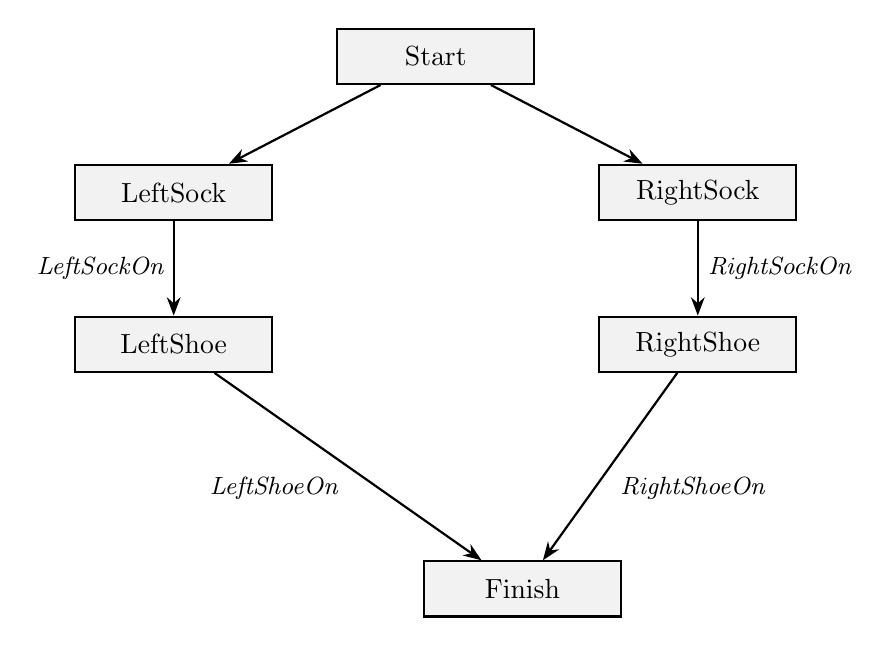
\begin{tikzpicture}[node distance=1.2cm and 2cm, >=Stealth, 
		action/.style={rectangle, draw=black, fill=gray!10, thick, minimum width=2.5cm, minimum height=0.7cm, align=center}]
		
		\node[action] (start) {Start};
		\node[action, below left=1cm and 0.8cm of start] (lsock) {LeftSock};
		\node[action, below right=1cm and 0.8cm of start] (rsock) {RightSock};
		\node[action, below=1.2cm of lsock] (lshoe) {LeftShoe};
		\node[action, below=1.2cm of rsock] (rshoe) {RightShoe};
		\node[action, below=1.2cm of lshoe] (finish) at (1.1, -5.2) {Finish};
		
		\draw[->, thick] (start) -- (lsock);
		\draw[->, thick] (start) -- (rsock);
		\draw[->, thick] (lsock) -- node[left, font=\small\itshape] {LeftSockOn} (lshoe);
		\draw[->, thick] (rsock) -- node[right, font=\small\itshape] {RightSockOn} (rshoe);
		\draw[->, thick] (lshoe) -- node[below left, font=\small\itshape] {LeftShoeOn} (finish);
		\draw[->, thick] (rshoe) -- node[below right, font=\small\itshape] {RightShoeOn} (finish);
	\end{tikzpicture}
\end{center}

\begin{enumerate}
	\item[\textbf{Parte 1.}] Faça uma descrição dos operadores:
	\begin{itemize}
		\item \textit{LeftSock} (colocar a meia no pé esquerdo)
		\item \textit{LeftShoe} (colocar o sapato no pé esquerdo)
		\item \textit{RightSock} (colocar a meia no pé direito)
		\item \textit{RightShoe} (colocar o sapato no pé direito)
	\end{itemize}
	\item[\textbf{Parte 2.}] Mostre passo a passo a construção do plano acima utilizando o algoritmo POP.
\end{enumerate}


\subsection*{Resposta:}

\bigskip


\subsection*{(Parte 1) Descrição Formal dos Operadores STRIPS/PDDL}

Para calçar o sapato é pré-requisito necessário que a meia correspondente já esteja calçada no mesmo pé. O estado inicial assume que ambos os pés estão sem meias e sem sapatos.

\subsubsection*{1. Action: LeftSock}
\begin{itemize}
	\item \textbf{PRECOND:} \textit{BareFoot(Left)} (pé esquerdo sem meia)
	\item \textbf{EFFECT:} \textit{LeftSockOn} $\wedge \neg \textit{BareFoot(Left)}$
\end{itemize}

\subsubsection*{2. Action: LeftShoe}
\begin{itemize}
	\item \textbf{PRECOND:} \textit{LeftSockOn}
	\item \textbf{EFFECT:} \textit{LeftShoeOn}
\end{itemize}

\subsubsection*{3. Action: RightSock}
\begin{itemize}
	\item \textbf{PRECOND:} \textit{BareFoot(Right)} (pé direito sem meia)
	\item \textbf{EFFECT:} \textit{RightSockOn} $\wedge \neg \textit{BareFoot(Right)}$
\end{itemize}

\subsubsection*{4. Action: RightShoe}
\begin{itemize}
	\item \textbf{PRECOND:} \textit{RightSockOn}
	\item \textbf{EFFECT:} \textit{RightShoeOn}
\end{itemize}

---

\subsection*{(Parte 2) Construção Passo a Passo pelo Algoritmo POP}

O algoritmo de **Planejamento de Ordem Parcial (POP)** opera regressivamente a partir do objetivo (\textit{Goal Regression}), adicionando ações para satisfazer precondições em aberto (\textit{open preconditions}) e garantindo que não haja ameaças de ordem causal.

\subsubsection*{Passo 0: Inicialização do Plano Incompleto}
\begin{itemize}
	\item \textbf{Ação Inicial ($Start$):} Efeitos = $\{\textit{BareFoot(Left)}, \textit{BareFoot(Right)}\}$
	\item \textbf{Ação Final ($Finish$):} Precondições = $\{\textit{LeftShoeOn}, \textit{RightShoeOn}\}$
	\item \textbf{Ordenação Inicial:} $Start < Finish$
	\item \textbf{Precondições em Aberto:} $(\textit{LeftShoeOn}, Finish)$, $(\textit{RightShoeOn}, Finish)$
\end{itemize}

\subsubsection*{Passo 1: Resolver a Precondição em Aberto $(\textit{LeftShoeOn}, Finish)$}
\begin{itemize}
	\item Seleciona a ação $\textit{LeftShoe}$, cujos efeitos satisfazem $\textit{LeftShoeOn}$.
	\item Adiciona o elo causal (\textit{Causal Link}): $\textit{LeftShoe} \xrightarrow{\textit{LeftShoeOn}} Finish$.
	\item Adiciona as ordenações necessárias: $Start < \textit{LeftShoe} < Finish$.
	\item **Nova precondição em aberto criada:** $(\textit{LeftSockOn}, \textit{LeftShoe})$.
\end{itemize}

\subsubsection*{Passo 2: Resolver a Precondição em Aberto $(\textit{RightShoeOn}, Finish)$}
\begin{itemize}
	\item Seleciona a ação $\textit{RightShoe}$, cujos efeitos satisfazem $\textit{RightShoeOn}$.
	\item Adiciona o elo causal: $\textit{RightShoe} \xrightarrow{\textit{RightShoeOn}} Finish$.
	\item Adiciona as ordenações: $Start < \textit{RightShoe} < Finish$.
	\item **Nova precondição em aberto criada:** $(\textit{RightSockOn}, \textit{RightShoe})$.
\end{itemize}

\subsubsection*{Passo 3: Resolver a Precondição em Aberto $(\textit{LeftSockOn}, \textit{LeftShoe})$}
\begin{itemize}
	\item Seleciona a ação $\textit{LeftSock}$, que produz o efeito $\textit{LeftSockOn}$.
	\item Adiciona o elo causal: $\textit{LeftSock} \xrightarrow{\textit{LeftSockOn}} \textit{LeftShoe}$.
	\item Conecta a precondição de $\textit{LeftSock}$ ($\textit{BareFoot(Left)}$) diretamente ao estado $Start$: $Start \xrightarrow{\textit{BareFoot(Left)}} \textit{LeftSock}$.
\end{itemize}

\subsubsection*{Passo 4: Resolver a Precondição em Aberto $(\textit{RightSockOn}, \textit{RightShoe})$}
\begin{itemize}
	\item Seleciona a ação $\textit{RightSock}$, que produz o efeito $\textit{RightSockOn}$.
	\item Adiciona o elo causal: $\textit{RightSock} \xrightarrow{\textit{RightSockOn}} \textit{RightShoe}$.
	\item Conecta a precondição de $\textit{RightSock}$ ($\textit{BareFoot(Right)}$) diretamente ao estado $Start$: $Start \xrightarrow{\textit{BareFoot(Right)}} \textit{RightSock}$.
\end{itemize}

\subsubsection*{Passo 5: Verificação de Ameaças (\textit{Threat Checking})}
\begin{itemize}
	\item O algoritmo verifica se alguma ação ameaça destruir os elos causais estabelecidos.
	\item Como as cadeias para o pé esquerdo ($\textit{LeftSock} \to \textit{LeftShoe}$) e para o pé direito ($\textit{RightSock} \to \textit{RightShoe}$) utilizam recursos totalmente independentes, **não existem conflitos nem ameaças** entre os dois ramos.
	\item As ações dos dois lados podem ser intercaladas em qualquer ordem válida no plano final (ex: $\text{LeftSock} \to \text{RightSock} \to \text{LeftShoe} \to \text{RightShoe}$ ou vice-versa).
\end{itemize}

---

\subsection*{Grafo da Solução Final (Grafo POP)}

A estrutura gráfica resultante do plano de ordem parcial construído é ilustrada no grafo a seguir:

\begin{center}
	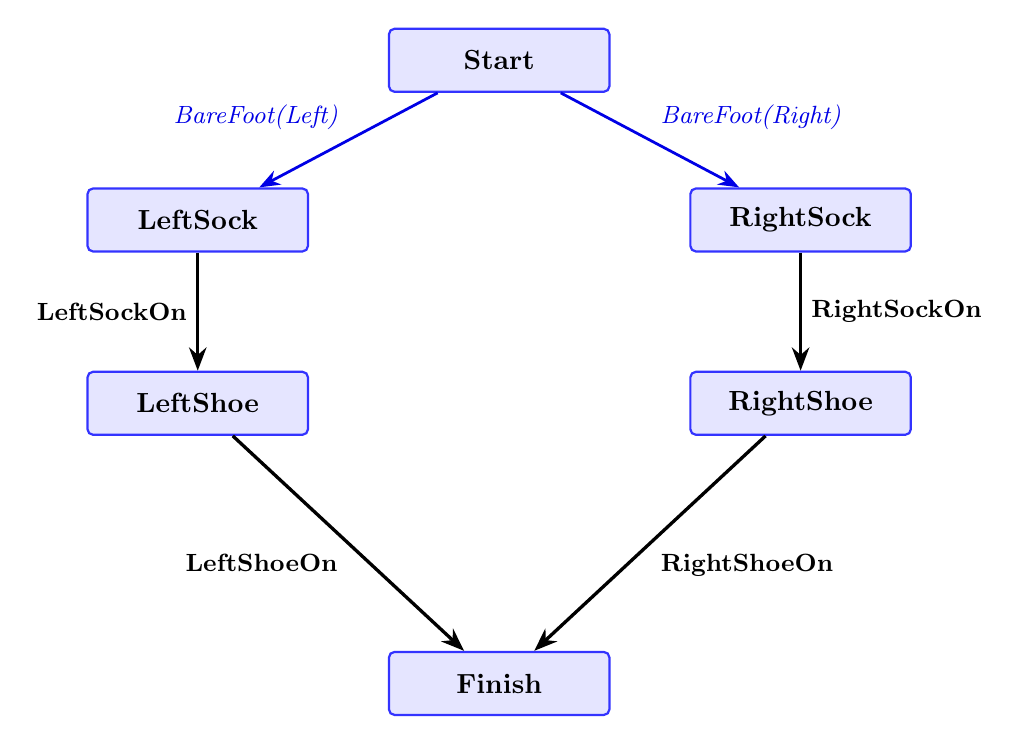
\begin{tikzpicture}[node distance=1.5cm and 2.5cm, >=Stealth, 
		action/.style={rectangle, draw=blue!80, fill=blue!10, thick, minimum width=2.8cm, minimum height=0.8cm, align=center, rounded corners=2pt}]
		
		\node[action] (start) {\textbf{Start}};
		\node[action, below left=1.2cm and 1cm of start] (lsock) {\textbf{LeftSock}};
		\node[action, below right=1.2cm and 1cm of start] (rsock) {\textbf{RightSock}};
		\node[action, below=1.5cm of lsock] (lshoe) {\textbf{LeftShoe}};
		\node[action, below=1.5cm of rsock] (rshoe) {\textbf{RightShoe}};
		\node[action, below=1.5cm of lshoe] (finish) at (0, -6.0) {\textbf{Finish}};
		
		\draw[->, line width=1pt, color=blue!90!black] (start) -- node[above left, font=\small\itshape] {BareFoot(Left)} (lsock);
		\draw[->, line width=1pt, color=blue!90!black] (start) -- node[above right, font=\small\itshape] {BareFoot(Right)} (rsock);
		
		\draw[->, line width=1.2pt, color=black] (lsock) -- node[left, font=\small\bfseries] {LeftSockOn} (lshoe);
		\draw[->, line width=1.2pt, color=black] (rsock) -- node[right, font=\small\bfseries] {RightSockOn} (rshoe);
		
		\draw[->, line width=1.2pt, color=black] (lshoe) -- node[below left, font=\small\bfseries] {LeftShoeOn} (finish);
		\draw[->, line width=1.2pt, color=black] (rshoe) -- node[below right, font=\small\bfseries] {RightShoeOn} (finish);
	\end{tikzpicture}
\end{center}


\section*{Questão 17}

Considere o problema de planejamento com 2 ações, $A_1$ e $A_2$. A ação $A_1$ tem precondição $q$ e efeitos $\{p, \neg q\}$. A ação $A_2$ não tem precondições e tem efeito $r$. O estado inicial é $\{q\}$. A meta é $\{p, r\}$. O grafo de planejamento expandido (gerado pelo algoritmo GRAPHPLAN) até o nível 1, sem marcações de mutexes, é dado a seguir:

\begin{center}
	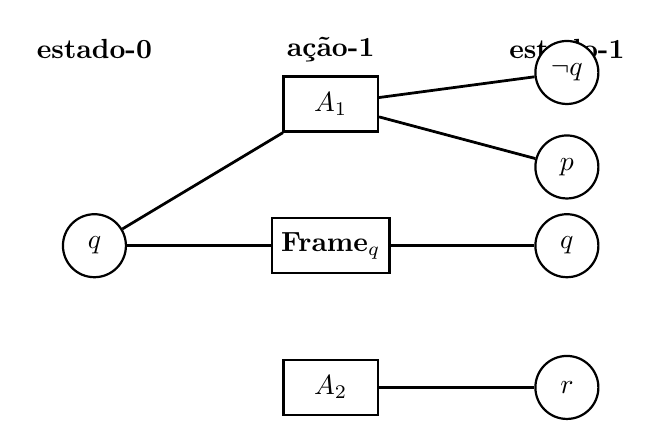
\begin{tikzpicture}[node distance=1.5cm and 2.5cm, >=Stealth, 
		state/.style={circle, draw=black, fill=white, thick, minimum size=0.8cm, font=\bfseries},
		action/.style={rectangle, draw=black, fill=white, thick, minimum width=1.2cm, minimum height=0.7cm, font=\bfseries}]
		
		% Títulos dos Níveis
		\node (s0_t) at (0, 2.5) {\textbf{estado-0}};
		\node (a1_t) at (3, 2.5) {\textbf{ação-1}};
		\node (s1_t) at (6, 2.5) {\textbf{estado-1}};
		
		% Estado 0
		\node[state] (q0) at (0, 0) {$q$};
		
		% Ações Nível 1
		\node[action] (a1) at (3, 1.8) {$A_1$};
		\node[action] (frame_q) at (3, 0) {$\text{Frame}_q$};
		\node[action] (a2) at (3, -1.8) {$A_2$};
		
		% Estado 1
		\node[state] (notq1) at (6, 2.2) {$\neg q$};
		\node[state] (p1) at (6, 1.0) {$p$};
		\node[state] (q1) at (6, 0) {$q$};
		\node[state] (r1) at (6, -1.8) {$r$};
		
		% Arestas Precondições (S0 -> A1)
		\draw[line width=1pt] (q0) -- (a1);
		\draw[line width=1pt] (q0) -- (frame_q);
		% A2 não tem precondição (sem linha vinda de q0)
		
		% Arestas Efeitos (A1 -> S1)
		\draw[line width=1pt] (a1) -- (notq1);
		\draw[line width=1pt] (a1) -- (p1);
		\draw[line width=1pt] (frame_q) -- (q1);
		\draw[line width=1pt] (a2) -- (r1);
	\end{tikzpicture}
\end{center}

\begin{enumerate}
	\item[\textbf{PARTE 1:}] Marque os mutexes no grafo de planejamento (Nível 1).
	\item[\textbf{PARTE 2:}] Estenda o grafo até o segundo nível (níveis ação-2 e estado-2) e complete a marcação dos demais mutexes.
	\item[\textbf{PARTE 3:}] Mostre um plano válido (subgrafo) que corresponda a uma solução.
\end{enumerate}



\subsection*{Resposta:}

\bigskip

\subsection*{(PARTE 1) Marcação de Mutexes no Nível 1}

Analisando as regras de exclusão mútua do Graphplan para a estrutura do enunciado:

\subsubsection*{Mutexes entre Ações (Nível Ação-1):}
\begin{enumerate}
	\item $\text{Mutex}(A_1, \text{Frame}_q)$: \textbf{Interferência / Efeitos Inconsistentes}. $A_1$ produz $\neg q$, destruindo o efeito e a precondição $q$ mantidos pela persistência $\text{Frame}_q$.
	\item $\text{Mutex}(A_1, A_2)$: \textbf{NÃO são mutex}! $A_1$ exige $q$ e gera $\{p, \neg q\}$, enquanto $A_2$ não tem precondição e gera $r$. Nenhuma ação interfere na precondição ou efeito da outra.
	\item $\text{Frame}_q$ e $A_2$: \textbf{NÃO são mutex}.
\end{enumerate}

\subsubsection*{Mutexes entre Literais (Nível Estado-1):}
\begin{enumerate}
	\item $\text{Mutex}(q, \neg q)$: \textbf{Literais Complementares}.
	\item $\text{Mutex}(p, q)$: \textbf{Suportes Inconsistentes}. A única ação que produz $p$ é $A_1$, e a única ação que produz $q$ é $\text{Frame}_q$. Como $\text{Mutex}(A_1, \text{Frame}_q)$, $p$ e $q$ são mutex.
	\item $\text{Mutex}(p, r)$: \textbf{NÃO SÃO MUTEX}! Como $A_1$ (que produz $p$) e $A_2$ (que produz $r$) NÃO são mutex no nível ação-1, os literais $p$ e $r$ já podem ser obtidos juntos sem conflito no **estado-1**!
\end{enumerate}

---

\subsection*{(PARTE 2) Expansão do Grafo para o Nível 2}

Como as ações $A_1$ e $A_2$ são independentes e não-conflitantes no nível ação-1, o conjunto meta $\{p, r\}$ já se torna **livre de mutex no estado-1**. 

\subsubsection*{Grafo de Planejamento Expandido até o Nível 2 com Marcações (TikZ):}

\begin{center}
	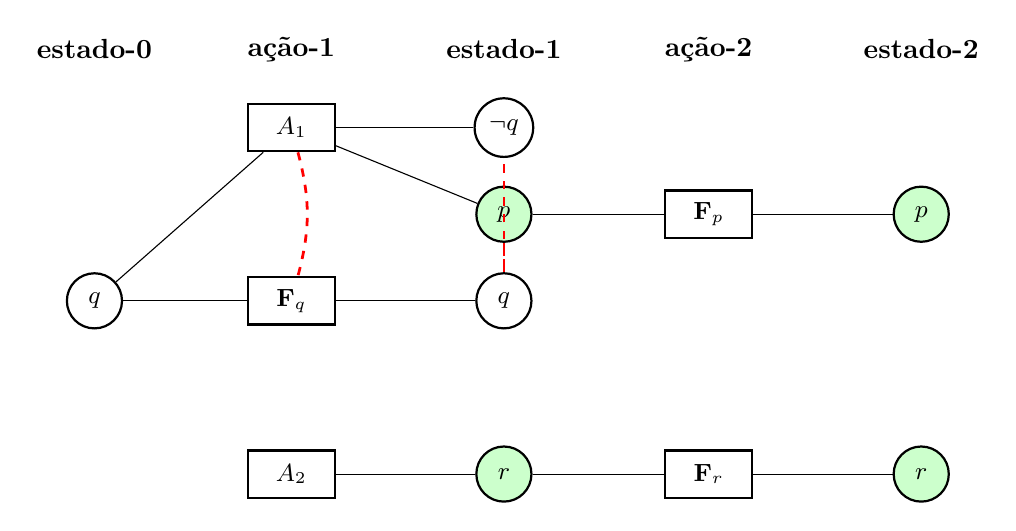
\begin{tikzpicture}[node distance=1.2cm and 2cm, >=Stealth, 
		state/.style={circle, draw=black, fill=white, thick, minimum size=0.7cm, font=\small\bfseries},
		action/.style={rectangle, draw=black, fill=white, thick, minimum width=1.1cm, minimum height=0.6cm, font=\small\bfseries},
		mutex/.style={red, dashed, line width=1pt}]
		
		% Títulos
		\node at (0, 3.2) {\textbf{estado-0}};
		\node at (2.5, 3.2) {\textbf{ação-1}};
		\node at (5.2, 3.2) {\textbf{estado-1}};
		\node at (7.8, 3.2) {\textbf{ação-2}};
		\node at (10.5, 3.2) {\textbf{estado-2}};
		
		% S0
		\node[state] (q0) at (0, 0) {$q$};
		
		% A1
		\node[action] (a1_1) at (2.5, 2.2) {$A_1$};
		\node[action] (fq1) at (2.5, 0) {$\text{F}_q$};
		\node[action] (a2_1) at (2.5, -2.2) {$A_2$};
		
		% S1
		\node[state] (notq1) at (5.2, 2.2) {$\neg q$};
		\node[state, fill=green!20] (p1) at (5.2, 1.1) {$p$};
		\node[state] (q1) at (5.2, 0) {$q$};
		\node[state, fill=green!20] (r1) at (5.2, -2.2) {$r$};
		
		% A2
		\node[action] (fp2) at (7.8, 1.1) {$\text{F}_p$};
		\node[action] (fr2) at (7.8, -2.2) {$\text{F}_r$};
		
		% S2
		\node[state, fill=green!20] (p2) at (10.5, 1.1) {$p$};
		\node[state, fill=green!20] (r2) at (10.5, -2.2) {$r$};
		
		% Arestas S0 -> A1
		\draw (q0) -- (a1_1);
		\draw (q0) -- (fq1);
		
		% Arestas A1 -> S1
		\draw (a1_1) -- (notq1);
		\draw (a1_1) -- (p1);
		\draw (fq1) -- (q1);
		\draw (a2_1) -- (r1);
		
		% Arestas S1 -> A2
		\draw (p1) -- (fp2);
		\draw (r1) -- (fr2);
		
		% Arestas A2 -> S2
		\draw (fp2) -- (p2);
		\draw (fr2) -- (r2);
		
		% Linhas Mutex Nível 1
		\draw[mutex] (a1_1) to[bend left=15] node[right, font=\tiny] {} (fq1);
		\draw[mutex] (q1) -- (notq1);
		\draw[mutex] (p1) -- (q1);
		
	\end{tikzpicture}
\end{center}

---

\subsection*{(PARTE 3) Busca Regressiva e Subgrafo Solução}

Realizando a busca de plano (\textit{Backward Search}) no estado-1 a partir da meta $\{p, r\}$:

1. No **nível ação-1**, selecionamos:
* Ação $A_1$ para gerar $p$ (requer a precondição $q$ no estado-0).
* Ação $A_2$ para gerar $r$ (não requer precondições).
2. Como $A_1$ e $A_2$ não possuem conflito de mutex entre si, ambas podem ser executadas **em paralelo no mesmo passo temporal (nível 1)**.

\subsubsection*{Plano Solução Extraído:}
O plano paralelo obtido no primeiro passo é:
\begin{equation}
	\mathbf{\text{Plano Solução}} = \big[ \{A_1, A_2\} \big]
\end{equation}

Se for exigido um plano estritamente sequencial (uma ação por vez), qualquer ordem de execução entre $A_1$ e $A_2$ é válida:
\begin{equation}
	\mathbf{\text{Plano Sequencial}} = \langle A_1, A_2 \rangle \quad \text{ou} \quad \langle A_2, A_1 \rangle
\end{equation}

\subsubsection*{Subgrafo Solução (TikZ):}

\begin{center}
	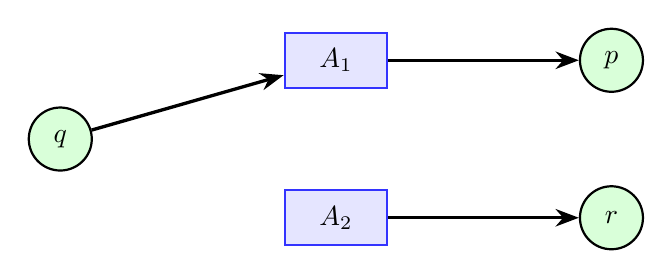
\begin{tikzpicture}[node distance=1.5cm and 2.5cm, >=Stealth, 
		state/.style={circle, draw=black, fill=green!15, thick, minimum size=0.8cm, font=\bfseries},
		action/.style={rectangle, draw=blue!80, fill=blue!10, thick, minimum width=1.3cm, minimum height=0.7cm, font=\bfseries}]
		
		\node[state] (q0) at (0, 0) {$q$};
		
		\node[action] (a1) at (3.5, 1) {$A_1$};
		\node[action] (a2) at (3.5, -1) {$A_2$};
		
		\node[state] (p1) at (7, 1) {$p$};
		\node[state] (r1) at (7, -1) {$r$};
		
		\draw[->, line width=1.2pt] (q0) -- (a1);
		\draw[->, line width=1.2pt] (a1) -- (p1);
		\draw[->, line width=1.2pt] (a2) -- (r1);
		
	\end{tikzpicture}
\end{center}


\section*{Questão 18}


Construa os níveis 0, 1 e 2 do grafo de planejamento para o problema da Figura 10.1 (Transporte de Carga Aérea).

\textbf{Definição PDDL do Problema (Figura 10.1):}
\begin{itemize}
	\item \textbf{Init:} $\text{At}(C_1, \text{SFO}) \wedge \text{At}(C_2, \text{JFK}) \wedge \text{At}(P_1, \text{SFO}) \wedge \text{At}(P_2, \text{JFK}) \wedge \text{Cargo}(C_1) \wedge \text{Cargo}(C_2) \wedge \text{Plane}(P_1) \wedge \text{Plane}(P_2) \wedge \text{Airport}(\text{JFK}) \wedge \text{Airport}(\text{SFO})$
	\item \textbf{Goal:} $\text{At}(C_1, \text{JFK}) \wedge \text{At}(C_2, \text{SFO})$
	\item \textbf{Action} $\text{Load}(c, p, a)$:
	\begin{itemize}
		\item \textbf{PRECOND:} $\text{At}(c, a) \wedge \text{At}(p, a) \wedge \text{Cargo}(c) \wedge \text{Plane}(p) \wedge \text{Airport}(a)$
		\item \textbf{EFFECT:} $\neg \text{At}(c, a) \wedge \text{In}(c, p)$
	\end{itemize}
	\item \textbf{Action} $\text{Unload}(c, p, a)$:
	\begin{itemize}
		\item \textbf{PRECOND:} $\text{In}(c, p) \wedge \text{At}(p, a) \wedge \text{Cargo}(c) \wedge \text{Plane}(p) \wedge \text{Airport}(a)$
		\item \textbf{EFFECT:} $\text{At}(c, a) \wedge \neg \text{In}(c, p)$
	\end{itemize}
	\item \textbf{Action} $\text{Fly}(p, \text{from}, \text{to})$:
	\begin{itemize}
		\item \textbf{PRECOND:} $\text{At}(p, \text{from}) \wedge \text{Plane}(p) \wedge \text{Airport}(\text{from}) \wedge \text{Airport}(\text{to})$
		\item \textbf{EFFECT:} $\neg \text{At}(p, \text{from}) \wedge \text{At}(p, \text{to})$
	\end{itemize}
\end{itemize}


\subsection*{Resposta:}

\bigskip


No Grafo de Planejamento (*Planning Graph*), omitimos os predicados estáticos de tipo (como $\text{Cargo}$, $\text{Plane}$, $\text{Airport}$) para focar nos fluentes de estado ($\text{At}$ e $\text{In}$).

\subsection*{Nível 0: Estado Inicial ($S_0$)}
O conjunto de literais fluentes presentes no nível de estado $S_0$ consiste em:
\begin{equation}
	S_0 = \{ \text{At}(C_1, \text{SFO}), \, \text{At}(P_1, \text{SFO}), \, \text{At}(C_2, \text{JFK}), \, \text{At}(P_2, \text{JFK}) \}
\end{equation}
\textit{Nota:} Não há relações de mutex no estado $S_0$.

---

\subsection*{Nível 1: Ações ($A_1$) e Estados ($S_1$)}

\subsubsection*{Ações Aplicáveis no Nível $A_1$:}
Com base nas precondições satisfeitas em $S_0$:
\begin{enumerate}
	\item \textbf{Carregamentos de Carga:}
	\begin{itemize}
		\item $\text{Load}(C_1, P_1, \text{SFO})$ (produz $\text{In}(C_1, P_1)$ e $\neg \text{At}(C_1, \text{SFO})$)
		\item $\text{Load}(C_2, P_2, \text{JFK})$ (produz $\text{In}(C_2, P_2)$ e $\neg \text{At}(C_2, \text{JFK})$)
	\end{itemize}
	
	\item \textbf{Voos de Aviões:}
	\begin{itemize}
		\item $\text{Fly}(P_1, \text{SFO}, \text{JFK})$ (produz $\text{At}(P_1, \text{JFK})$ e $\neg \text{At}(P_1, \text{SFO})$)
		\item $\text{Fly}(P_2, \text{JFK}, \text{SFO})$ (produz $\text{At}(P_2, \text{SFO})$ e $\neg \text{At}(P_2, \text{JFK})$)
	\end{itemize}
	
	\item \textbf{Ações de Persistência ($\text{Frame}$):}
	\begin{itemize}
		\item $\text{Frame}_{\text{At}(C_1, \text{SFO})}, \, \text{Frame}_{\text{At}(P_1, \text{SFO})}, \, \text{Frame}_{\text{At}(C_2, \text{JFK})}, \, \text{Frame}_{\text{At}(P_2, \text{JFK})}$
	\end{itemize}
\end{enumerate}

\subsubsection*{Principais Mutexes no Nível Ação $A_1$:}
\begin{itemize}
	\item $\text{Mutex}(\text{Load}(C_1, P_1, \text{SFO}), \, \text{Fly}(P_1, \text{SFO}, \text{JFK}))$: \textbf{Interferência / Efeitos Inconsistentes} ($\text{Fly}$ remove a precondição/efeito $\text{At}(P_1, \text{SFO})$).
	\item $\text{Mutex}(\text{Load}(C_1, P_1, \text{SFO}), \, \text{Frame}_{\text{At}(C_1, \text{SFO})})$: \textbf{Efeitos Inconsistentes} ($\text{Load}$ apaga $\text{At}(C_1, \text{SFO})$).
	\item $\text{Mutex}(\text{Fly}(P_1, \text{SFO}, \text{JFK}), \, \text{Frame}_{\text{At}(P_1, \text{SFO})})$: \textbf{Efeitos Inconsistentes}.
\end{itemize}

\subsubsection*{Conjunto de Literais no Estado $S_1$:}
\begin{align*}
	S_1 = \{ & \text{At}(C_1, \text{SFO}), \, \text{At}(P_1, \text{SFO}), \, \text{At}(C_2, \text{JFK}), \, \text{At}(P_2, \text{JFK}), \\
	& \text{In}(C_1, P_1), \, \text{In}(C_2, P_2), \, \text{At}(P_1, \text{JFK}), \, \text{At}(P_2, \text{SFO}), \, \neg \text{At}(C_1, \text{SFO}), \dots \}
\end{align*}

---

\subsection*{Nível 2: Ações ($A_2$) e Estados ($S_2$)}

No nível $A_2$, surgem as ações de descarregamento ($\text{Unload}$), pois a precondição $\text{In}(c, p)$ agora existe em $S_1$.

\subsubsection*{Novas Ações Aplicáveis no Nível $A_2$:}
\begin{itemize}
	\item $\text{Unload}(C_1, P_1, \text{JFK})$ (requer $\text{In}(C_1, P_1)$ e $\text{At}(P_1, \text{JFK})$ $\to$ produz $\text{At}(C_1, \text{JFK})$)
	\item $\text{Unload}(C_2, P_2, \text{SFO})$ (requer $\text{In}(C_2, P_2)$ e $\text{At}(P_2, \text{SFO})$ $\to$ produz $\text{At}(C_2, \text{SFO})$)
	\item Diversas novas ações de voo e carregamento em novos locais, além das ações de persistência.
\end{itemize}

\subsubsection*{Saturação da Meta em $S_2$:}
No nível de estado $S_2$, os literais da meta $\{\text{At}(C_1, \text{JFK}), \, \text{At}(C_2, \text{SFO})\}$ aparecem produzidos por $\text{Unload}(C_1, P_1, \text{JFK})$ e $\text{Unload}(C_2, P_2, \text{SFO})$. Como essas duas ações pertencem a subredes independentes ($P_1/C_1$ vs $P_2/C_2$), elas **não são mutex**, permitindo alcançar a meta!

---

\subsection*{Grafo de Planejamento Expandido (Níveis 0, 1 e 2 em TikZ)}

\begin{center}
	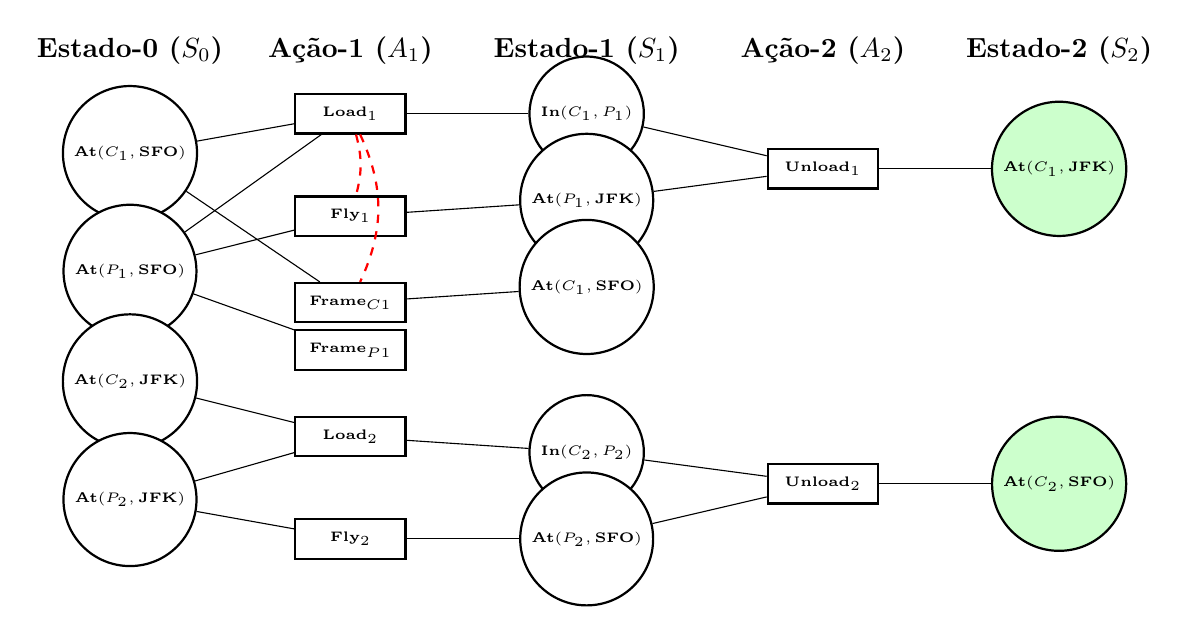
\begin{tikzpicture}[node distance=1.1cm and 2.2cm, >=Stealth, 
		state/.style={circle, draw=black, fill=white, thick, minimum size=0.6cm, font=\tiny\bfseries},
		action/.style={rectangle, draw=black, fill=white, thick, minimum width=1.4cm, minimum height=0.5cm, font=\tiny\bfseries},
		mutex/.style={red, dashed, line width=0.8pt}]
		
		% Títulos
		\node at (0, 3.5) {\textbf{Estado-0 ($S_0$)}};
		\node at (2.8, 3.5) {\textbf{Ação-1 ($A_1$)}};
		\node at (5.8, 3.5) {\textbf{Estado-1 ($S_1$)}};
		\node at (8.8, 3.5) {\textbf{Ação-2 ($A_2$)}};
		\node at (11.8, 3.5) {\textbf{Estado-2 ($S_2$)}};
		
		% S0 Nodes
		\node[state] (ac1_sfo_0) at (0, 2.2) {$\text{At}(C_1,\text{SFO})$};
		\node[state] (ap1_sfo_0) at (0, 0.7) {$\text{At}(P_1,\text{SFO})$};
		\node[state] (ac2_jfk_0) at (0, -0.7) {$\text{At}(C_2,\text{JFK})$};
		\node[state] (ap2_jfk_0) at (0, -2.2) {$\text{At}(P_2,\text{JFK})$};
		
		% A1 Nodes
		\node[action] (load1_1) at (2.8, 2.7) {$\text{Load}_1$};
		\node[action] (fly1_1) at (2.8, 1.4) {$\text{Fly}_1$};
		\node[action] (f_ac1) at (2.8, 0.3) {$\text{Frame}_{C1}$};
		\node[action] (f_ap1) at (2.8, -0.3) {$\text{Frame}_{P1}$};
		\node[action] (load2_1) at (2.8, -1.4) {$\text{Load}_2$};
		\node[action] (fly2_1) at (2.8, -2.7) {$\text{Fly}_2$};
		
		% S1 Nodes
		\node[state] (in1_p1_1) at (5.8, 2.7) {$\text{In}(C_1,P_1)$};
		\node[state] (ap1_jfk_1) at (5.8, 1.6) {$\text{At}(P_1,\text{JFK})$};
		\node[state] (ac1_sfo_1) at (5.8, 0.5) {$\text{At}(C_1,\text{SFO})$};
		\node[state] (in2_p2_1) at (5.8, -1.6) {$\text{In}(C_2,P_2)$};
		\node[state] (ap2_sfo_1) at (5.8, -2.7) {$\text{At}(P_2,\text{SFO})$};
		
		% A2 Nodes
		\node[action] (unload1_2) at (8.8, 2.0) {$\text{Unload}_1$};
		\node[action] (unload2_2) at (8.8, -2.0) {$\text{Unload}_2$};
		
		% S2 Nodes
		\node[state, fill=green!20] (ac1_jfk_2) at (11.8, 2.0) {$\text{At}(C_1,\text{JFK})$};
		\node[state, fill=green!20] (ac2_sfo_2) at (11.8, -2.0) {$\text{At}(C_2,\text{SFO})$};
		
		% Links S0 -> A1
		\draw (ac1_sfo_0) -- (load1_1);
		\draw (ap1_sfo_0) -- (load1_1);
		\draw (ap1_sfo_0) -- (fly1_1);
		\draw (ac1_sfo_0) -- (f_ac1);
		\draw (ap1_sfo_0) -- (f_ap1);
		
		\draw (ac2_jfk_0) -- (load2_1);
		\draw (ap2_jfk_0) -- (load2_1);
		\draw (ap2_jfk_0) -- (fly2_1);
		
		% Links A1 -> S1
		\draw (load1_1) -- (in1_p1_1);
		\draw (fly1_1) -- (ap1_jfk_1);
		\draw (f_ac1) -- (ac1_sfo_1);
		\draw (load2_1) -- (in2_p2_1);
		\draw (fly2_1) -- (ap2_sfo_1);
		
		% Links S1 -> A2
		\draw (in1_p1_1) -- (unload1_2);
		\draw (ap1_jfk_1) -- (unload1_2);
		\draw (in2_p2_1) -- (unload2_2);
		\draw (ap2_sfo_1) -- (unload2_2);
		
		% Links A2 -> S2
		\draw (unload1_2) -- (ac1_jfk_2);
		\draw (unload2_2) -- (ac2_sfo_2);
		
		% Mutexes Nível A1
		\draw[mutex] (load1_1) to[bend left=15] (fly1_1);
		\draw[mutex] (load1_1) to[bend left=25] (f_ac1);
		
	\end{tikzpicture}
\end{center}


\section*{Questão 19}


A Figura 10.4 mostra um problema de mundo de blocos conhecido como \textbf{Anomalia de Sussman}. O problema foi considerado anômalo porque os planejadores sem intercalações (\textit{non-interleaved planners}) do início da década de 1970 não conseguiram resolvê-lo. 

\begin{center}
	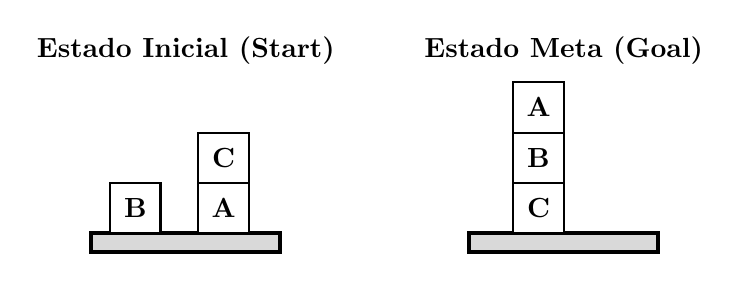
\begin{tikzpicture}[scale=0.8]
		% Start State
		\node at (1.5, 3.2) {\textbf{Estado Inicial (Start)}};
		% Mesa
		\draw[line width=1.5pt, fill=gray!30] (0, 0) rectangle (3, 0.3);
		% Blocos
		\draw[thick, fill=white] (0.3, 0.3) rectangle (1.1, 1.1) node[pos=.5, font=\bfseries] {B};
		\draw[thick, fill=white] (1.7, 0.3) rectangle (2.5, 1.1) node[pos=.5, font=\bfseries] {A};
		\draw[thick, fill=white] (1.7, 1.1) rectangle (2.5, 1.9) node[pos=.5, font=\bfseries] {C};
		
		% Goal State
		\node at (7.5, 3.2) {\textbf{Estado Meta (Goal)}};
		% Mesa
		\draw[line width=1.5pt, fill=gray!30] (6, 0) rectangle (9, 0.3);
		% Torre A-B-C
		\draw[thick, fill=white] (6.7, 0.3) rectangle (7.5, 1.1) node[pos=.5, font=\bfseries] {C};
		\draw[thick, fill=white] (6.7, 1.1) rectangle (7.5, 1.9) node[pos=.5, font=\bfseries] {B};
		\draw[thick, fill=white] (6.7, 1.9) rectangle (7.5, 2.7) node[pos=.5, font=\bfseries] {A};
	\end{tikzpicture}
\end{center}

Escreva uma definição do problema e resolva-o manualmente com o \textbf{Graphplan}. Um planejador sem intercalações é um planejador que, ao receber dois subobjetivos $G_1$ e $G_2$, produz um plano para $G_1$ concatenado com um plano para $G_2$ ou vice-versa. Explique por que um planejador sem intercalações não consegue resolver esse problema.


\subsection*{Resposta:}

\bigskip


\subsection*{1. Definição Formal do Problema (STRIPS / PDDL)}

\subsubsection*{Estado Inicial ($Init$):}
\begin{equation}
	Init = \{ \text{On}(C, A), \, \text{OnTable}(A), \, \text{OnTable}(B), \, \text{Clear}(C), \, \text{Clear}(B), \, \text{ArmEmpty} \}
\end{equation}

\subsubsection*{Estado Meta ($Goal$):}
\begin{equation}
	Goal = \{ \text{On}(A, B), \, \text{On}(B, C) \}
\end{equation}

---

\subsection*{2. Por que Planejadores Sem Intercalação Falham?}

Um planejador sem intercalação (*non-interleaved planner*, como o *STRIPS original*) tenta resolver a meta decompondo-a em subobjetivos independentes: $G_1 = \text{On}(A, B)$ e $G_2 = \text{On}(B, C)$, exigindo resolver completamente $G_1$ e depois $G_2$ (ou vice-versa):

\begin{enumerate}
	\item \textbf{Tentar resolver $G_1 = \text{On}(A, B)$ primeiro:}
	Para colocar $A$ sobre $B$, é necessário tirar $C$ de cima de $A$ (colocando $C$ na mesa) e então mover $A$ para cima de $B$. 
	\textit{Resultado parcial:} $A$ fica em cima de $B$. Mas para depois resolver $G_2 = \text{On}(B, C)$, $B$ precisa ser movido para cima de $C$, o que exige **desfazer** a conquista prévia de $\text{On}(A, B)$ (tirando $A$ de cima de $B$). O planejador entra em *loop* ou falha.
	
	\item \textbf{Tentar resolver $G_2 = \text{On}(B, C)$ primeiro:}
	Para colocar $B$ em cima de $C$, move-se $B$ para $C$. 
	\textit{Resultado parcial:} $B$ fica sobre $C$. Mas para depois resolver $G_1 = \text{On}(A, B)$, $A$ precisa ser colocado sobre $B$, mas $A$ ainda está preso embaixo de $C$! Para tirar $C$ de cima de $A$, $B$ terá que ser tirado do topo de $C$, desfazendo $G_2$.
\end{enumerate}

\textbf{Conclusão:} A resolução requer **intercalar** passos das duas metas: liberar $A$ primeiro (tirando $C$), depois resolver $G_2 = \text{On}(B, C)$, e por fim resolver $G_1 = \text{On}(A, B)$.

---

\subsection*{3. Resolução Passo a Passo com o Graphplan}

\subsubsection*{Nível 0 ($S_0$):}
$S_0 = \{ \text{On}(C, A), \, \text{OnTable}(A), \, \text{OnTable}(B), \, \text{Clear}(C), \, \text{Clear}(B) \}$

\subsubsection*{Nível 1 ($A_1 \to S_1$):}
Ações aplicáveis em $S_0$:
\begin{itemize}
	\item $\text{Unstack}(C, A) \to$ produz $\text{Holding}(C), \text{Clear}(A)$.
	\item Ações de Persistência ($\text{Frame}$).
\end{itemize}

\subsubsection*{Nível 2 ($A_2 \to S_2$):}
Com $\text{Holding}(C)$ e $\text{Clear}(A)$ disponíveis em $S_1$:
\begin{itemize}
	\item $\text{PutDown}(C) \to$ produz $\text{OnTable}(C), \text{Clear}(C), \text{ArmEmpty}$.
\end{itemize}

\subsubsection*{Nível 3 ($A_3 \to S_3$):}
Com $\text{ArmEmpty}, \text{Clear}(B)$ e $\text{Clear}(C)$ em $S_2$:
\begin{itemize}
	\item $\text{PickUp}(B) \to$ produz $\text{Holding}(B)$.
	\item $\text{Stack}(B, C) \to$ (no próximo passo) produz $\text{On}(B, C)$.
\end{itemize}

\subsubsection*{Nível 4 ($A_4 \to S_4$):}
Com $\text{On}(B, C), \text{Clear}(A)$ e $\text{ArmEmpty}$:
\begin{itemize}
	\item $\text{PickUp}(A) \to$ pega $A$ da mesa.
	\item $\text{Stack}(A, B) \to$ coloca $A$ em cima de $B$.
\end{itemize}

No estado $S_4$, a meta $\{\text{On}(A, B), \text{On}(B, C)\}$ é alcançada livre de mutexes!

---

\subsection*{4. Grafo de Planejamento da Solução (TikZ)}

O subgrafo solução extraído do Graphplan representa o plano correto de 3 passos de movimentação (além de desempilhar):

\begin{center}
	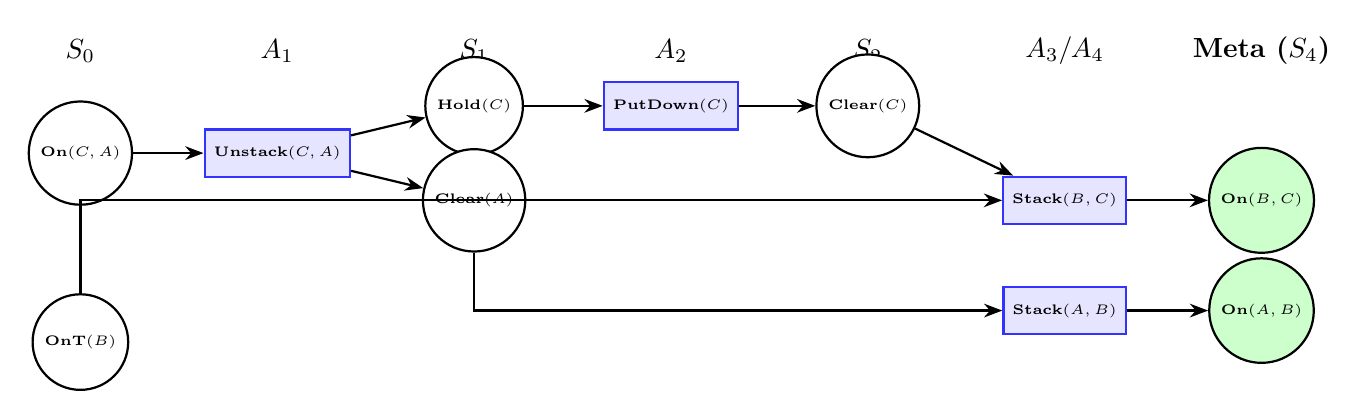
\begin{tikzpicture}[node distance=1.2cm and 2.2cm, >=Stealth, 
		state/.style={circle, draw=black, fill=white, thick, minimum size=0.6cm, font=\tiny\bfseries},
		action/.style={rectangle, draw=blue!80, fill=blue!10, thick, minimum width=1.4cm, minimum height=0.6cm, font=\tiny\bfseries}]
		
		% Titulos
		\node at (0, 2.5) {\textbf{$S_0$}};
		\node at (2.5, 2.5) {\textbf{$A_1$}};
		\node at (5.0, 2.5) {\textbf{$S_1$}};
		\node at (7.5, 2.5) {\textbf{$A_2$}};
		\node at (10.0, 2.5) {\textbf{$S_2$}};
		\node at (12.5, 2.5) {\textbf{$A_3/A_4$}};
		\node at (15.0, 2.5) {\textbf{Meta ($S_4$)}};
		
		% S0
		\node[state] (onca0) at (0, 1.2) {$\text{On}(C,A)$};
		\node[state] (tb0) at (0, -1.2) {$\text{OnT}(B)$};
		
		% A1
		\node[action] (unstack) at (2.5, 1.2) {$\text{Unstack}(C,A)$};
		
		% S1
		\node[state] (holdc) at (5.0, 1.8) {$\text{Hold}(C)$};
		\node[state] (cleara) at (5.0, 0.6) {$\text{Clear}(A)$};
		
		% A2
		\node[action] (putdown) at (7.5, 1.8) {$\text{PutDown}(C)$};
		
		% S2
		\node[state] (clearc) at (10.0, 1.8) {$\text{Clear}(C)$};
		
		% A3 / A4
		\node[action] (stackbc) at (12.5, 0.6) {$\text{Stack}(B,C)$};
		\node[action] (stackab) at (12.5, -0.8) {$\text{Stack}(A,B)$};
		
		% S4 Meta
		\node[state, fill=green!20] (onbc) at (15.0, 0.6) {$\text{On}(B,C)$};
		\node[state, fill=green!20] (onab) at (15.0, -0.8) {$\text{On}(A,B)$};
		
		% Arestas
		\draw[->, thick] (onca0) -- (unstack);
		\draw[->, thick] (unstack) -- (holdc);
		\draw[->, thick] (unstack) -- (cleara);
		\draw[->, thick] (holdc) -- (putdown);
		\draw[->, thick] (putdown) -- (clearc);
		
		\draw[->, thick] (clearc) -- (stackbc);
		\draw[->, thick] (tb0) |- (stackbc);
		\draw[->, thick] (cleara) |- (stackab);
		
		\draw[->, thick] (stackbc) -- (onbc);
		\draw[->, thick] (stackab) -- (onab);
		
	\end{tikzpicture}
\end{center}

\textbf{Plano Solução Extraído:}
\begin{equation}
	\mathbf{\text{Plano}} = \langle \text{Unstack}(C, A), \, \text{PutDown}(C), \, \text{Move}(B, \text{Table}, C), \, \text{Move}(A, \text{Table}, B) \rangle
\end{equation}


\section*{Questão 20}


\textbf{PARTE A:} Explique a ideia geral de extração automática de heurísticas de planejamento que fazem a relaxação dos efeitos negativos (Algoritmo do tipo Bellman--Ford, Aula 16, slides 16 e 22).

\bigskip

\textbf{PARTE B:} Explique as suposições feitas no cálculo das heurísticas $h_{\text{add}}^+(s)$ e $h_{\text{max}}^+(s)$ usando o algoritmo.


\subsection*{Resposta:}

\bigskip


\subsection*{PARTE A: Idéia Geral de Extração Automática de Heurísticas por Relaxação dos Efeitos Negativos ($P^+$)}

\subsubsection*{1. O Conceito da Relaxação $P^+$}
Na busca em planejamento clássico, calcular o custo exato do caminho mínimo $c^*(P)$ a partir de um estado $s$ até a meta $g$ é um problema intratável ($\text{PSPACE-completo}$). Para extrair funções heurísticas automaticamente a partir da própria descrição PDDL do problema, aplica-se a **relaxação da remoção de deletados ($P^+$)**:
\begin{itemize}
	\item Ignoram-se os efeitos negativos das ações (isto é, considera-se apenas a lista de efeitos positivos $effects^+(a)$).
	\item **Monotonicidade:** Uma vez que um átomo $p$ se torna verdadeiro em um estado, ele permanece verdadeiro para sempre.
	\item Se $c^*(P^+)$ é o custo ótimo do problema relaxado $P^+$, a heurística perfeita relaxada é $h^+(s) = c^*(P^+)$. Como $P^+$ é uma relaxação válida do problema original $P$, $h^+(s)$ é **admissível**.
\end{itemize}

\subsubsection*{2. Aproximação Polinomial via Programação Dinâmica (Algoritmo Bellman--Ford)}
Como calcular $h^+(s)$ de forma ótima ainda é NP-difícil, os algoritmos aproximam $h^+(s)$ atualizando iterativamente o custo estimado $h(p, s)$ para alcançar cada átomo $p \in \mathcal{P}$ a partir de $s$ através de um algoritmo de **ponto-fixo (Bellman--Ford)**:

\begin{enumerate}
	\item \textbf{Inicialização:}
	\begin{equation}
		h(p, s) = 
		\begin{cases}
			0, & \text{se } p \in s \\
			\infty, & \text{caso contrário}
		\end{cases}
	\end{equation}
	
	\item \textbf{Propagação do Ponto-Fixo (Slide 16 e Slide 22):}
	Repete-se a atualização para cada ação aplicável $a$ ($precond(a) \subseteq X$) e para cada $p \in effects^+(a)$ até que nenhum valor de $h(p, s)$ mude:
	\begin{equation}
		h(p, s) \leftarrow \min \left\{ h(p, s), \, 1 + \text{Cost}(precond(a), s) \right\}
	\end{equation}
	onde $\text{Cost}(precond(a), s)$ varia conforme a função heurística adotada ($h_{\text{add}}^+$ ou $h_{\text{max}}^+$).
\end{enumerate}

---

\subsection*{PARTE B: Suposições e Análise de $h_{\text{add}}^+(s)$ e $h_{\text{max}}^+(s)$}

As heurísticas $h_{\text{add}}^+(s)$ e $h_{\text{max}}^+(s)$ diferem na maneira como agregam os custos de múltiplos pré-requisitos para acionar uma ação e para satisfazer o conjunto final de metas $g = \{g_1, g_2, \dots, g_n\}$.

\subsubsection*{1. Heurística Aditiva: $h_{\text{add}}^+(s)$ (Slide 14 e 16)}

\begin{itemize}
	\item \textbf{Suposição de Independência de Submetas:}
	Assume que o custo para alcançar um conjunto de proposições $C$ é a **soma** dos custos individuais para alcançar cada proposição em $C$:
	\begin{equation}
		\text{Cost}_{\text{add}}(C, s) = \sum_{q \in C} h(q, s)
	\end{equation}
	\item \textbf{Regra de Atualização no Ponto-Fixo:}
	\begin{equation}
		h(p, s) \leftarrow \min \left\{ h(p, s), \, 1 + \sum_{q \in precond(a)} h(q, s) \right\}
	\end{equation}
	\item \textbf{Custo Final da Meta:}
	\begin{equation}
		h_{\text{add}}^+(s) = h(g, s) = \sum_{p \in g} h(p, s)
	\end{equation}
	\item \textbf{Propriedade e Qualidade (Slide 19):}
	\begin{itemize}
		\item **NÃO é Admissível:** Superestima o custo real em problemas onde ações sobrepostas/compartilhadas geram submetas simultaneamente (pois conta a mesma ação múltiplas vezes para alcançar submetas diferentes).
		\item **Desempenho:** É muito rápida e **extremamente informativa** para guiar a busca em problemas difíceis.
	\end{itemize}
\end{itemize}

\subsubsection*{2. Heurística Máxima: $h_{\text{max}}^+(s)$ (Slide 20 e 22)}

\begin{itemize}
	\item \textbf{Suposição de Paralelismo / Custo Crítico:}
	Assume que o custo para alcançar um conjunto de proposições $C$ é dominado estritamente pela submeta de **maior custo** (caminho crítico), assumindo paralelismo irrestrito no grafo:
	\begin{equation}
		\text{Cost}_{\text{max}}(C, s) = \max_{q \in C} h(q, s)
	\end{equation}
	\item \textbf{Regra de Atualização no Ponto-Fixo:}
	\begin{equation}
		h(p, s) \leftarrow \min \left\{ h(p, s), \, 1 + \max_{q \in precond(a)} h(q, s) \right\}
	\end{equation}
	\item \textbf{Custo Final da Meta:}
	\begin{equation}
		h_{\text{max}}^+(s) = h(g, s) = \max_{p \in g} h(p, s)
	\end{equation}
	\item \textbf{Propriedade e Qualidade (Slide 21):}
	\begin{itemize}
		\item **É Admissível:** Nunca superestima o custo do plano relaxado ótimo $h^+(s)$, pois $h_{\text{max}}^+(s) \le h^+(s) \le c^*(P)$.
		\item **Desempenho:** É **pouco informativa** (muito fraca), pois ignora o custo acumulado de ter que executar múltiplas ações para atingir submetas independentes.
	\end{itemize}
\end{itemize}

---

\subsection*{Tabela Comparativa Resumida (Slides 16 e 22)}

\begin{center}
	\begin{tabular}{|l|c|c|}
		\hline
		\textbf{Característica} & \textbf{Heurística $h_{\text{add}}^+(s)$} & \textbf{Heurística $h_{\text{max}}^+(s)$} \\ \hline
		\textbf{Agregação em $precond(a)$} & $\sum_{q \in precond(a)} h(q, s)$ & $\max_{q \in precond(a)} h(q, s)$ \\ \hline
		\textbf{Agregação na Meta $g$} & $\sum_{p \in g} h(p, s)$ & $\max_{p \in g} h(p, s)$ \\ \hline
		\textbf{Suposição de Submetas} & Totalmente Independentes & Paralelismo / Gargalo Máximo \\ \hline
		\textbf{Admissibilidade} & \textbf{Não} (pode superestimar) & \textbf{Sim} (sempre subestima) \\ \hline
		\textbf{Informatividade} & Alta (Guia bem a busca) & Baixa (Muitos empates) \\ \hline
	\end{tabular}
\end{center}

---

\subsection*{Ilustração Gráfica da Propagação de Custo (TikZ)}

O gráfico abaixo ilustra a diferença de cálculo entre $h_{\text{add}}^+$ e $h_{\text{max}}^+$ ao propagar os custos de um estado inicial $s = \{p_1, p_2\}$ através de uma ação $a$ com $precond(a) = \{p_1, p_2\}$ e $effects^+(a) = \{g_1\}$:

\begin{center}
	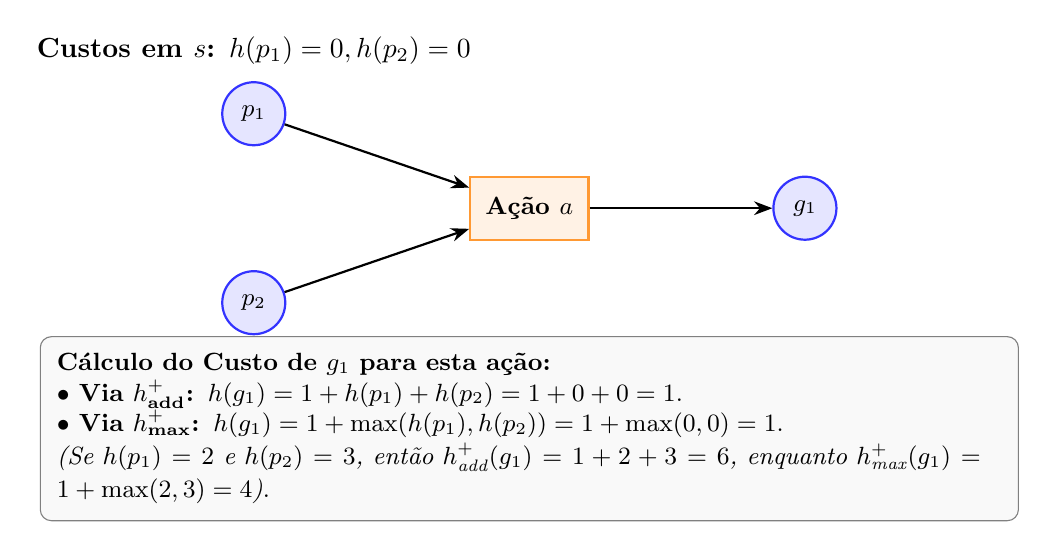
\begin{tikzpicture}[node distance=1.5cm and 2.5cm, >=Stealth, 
		atom/.style={circle, draw=blue!80, fill=blue!10, thick, minimum size=0.8cm, font=\small\bfseries},
		action/.style={rectangle, draw=orange!80, fill=orange!10, thick, minimum width=1.5cm, minimum height=0.8cm, font=\small\bfseries}]
		
		% Nos de entrada
		\node[atom] (p1) at (0, 1.2) {$p_1$};
		\node[atom] (p2) at (0, -1.2) {$p_2$};
		\node at (0, 2.0) {\textbf{Custos em $s$: $h(p_1)=0, h(p_2)=0$}};
		
		% Acao
		\node[action] (act) at (3.5, 0) {Ação $a$};
		
		% No de saida
		\node[atom] (g1) at (7, 0) {$g_1$};
		
		% Arestas
		\draw[->, thick] (p1) -- (act);
		\draw[->, thick] (p2) -- (act);
		\draw[->, thick] (act) -- (g1);
		
		% Caixa explicativa
		\node[draw=gray, fill=gray!5, rounded corners, inner sep=6pt, text width=12cm] at (3.5, -2.8) {
			\small
			\textbf{Cálculo do Custo de $g_1$ para esta ação:}\\
			$\bullet$ \textbf{Via $h_{\text{add}}^+$:} $h(g_1) = 1 + h(p_1) + h(p_2) = 1 + 0 + 0 = 1$.\\
			$\bullet$ \textbf{Via $h_{\text{max}}^+$:} $h(g_1) = 1 + \max(h(p_1), h(p_2)) = 1 + \max(0, 0) = 1$.\\
			\textit{(Se $h(p_1)=2$ e $h(p_2)=3$, então $h_{\text{add}}^+(g_1) = 1+2+3 = 6$, enquanto $h_{\text{max}}^+(g_1) = 1+\max(2,3) = 4$)}.
		};
		
	\end{tikzpicture}
\end{center}


\end{document}
